% !TEX program = pdflatex
\documentclass[14pt,russian]{scrartcl}
\let\counterwithout\relax
\let\counterwithin\relax
\usepackage{float}
\usepackage{xcolor}
\usepackage{extsizes}
\usepackage{subfig}
\usepackage[export]{adjustbox}
\usepackage[subfigure]{tocloft}
\usepackage[newfloat]{minted}
\newenvironment{longlisting}{\captionsetup{type=listing}}{}
\setminted{
  numbers=left,
  numbersep=5pt,
  fontsize=\footnotesize,
  breaklines=true,
  frame=single,
  xleftmargin=25pt,
  xrightmargin=25pt,
  framesep=3pt,
}
\makeatletter
\@removefromreset{listing}{section}
\@removefromreset{lstlisting}{section}
\makeatother
\renewcommand{\thelisting}{\arabic{listing}}
\AtBeginDocument{\renewcommand{\thelstlisting}{\arabic{lstlisting}}}
\usepackage[normalem]{ulem}
\usepackage{calc}
\usepackage{tabularx}
\usepackage{caption}
\DeclareCaptionLabelSeparator*{emdash}{~--- }
\captionsetup[listing]{position=top,labelsep=emdash,justification=raggedright,singlelinecheck=false,skip=0pt}
\captionsetup[lstlisting]{position=top,labelsep=emdash,justification=raggedright,singlelinecheck=false,skip=0pt}

\makeatletter
\AddToHook{begindocument/before}{\@ifpackageloaded{minted}{\removefromtoclist[float]{lol}}{}}
\makeatother


\usepackage{fancyvrb}
\usepackage{ulem,bm,mathrsfs,ifsym}

%%% Поля и разметка страницы %%%
\usepackage{pdflscape}
\usepackage{geometry}
\geometry{a4paper,tmargin=2cm,bmargin=2cm,lmargin=3cm,rmargin=1cm}

%%% Математические пакеты %%%
\usepackage{amsthm,amsfonts,amsmath,amssymb,amscd}
\usepackage{mathtools}
\usepackage[perpage]{footmisc}

\KOMAoptions{fontsize=14pt}

\makeatletter
\def\showfontsize{\f@size{} point}
\makeatother

\makeatletter
\setlength{\@fptop}{0pt}
\makeatother

\usepackage{tempora}
\usepackage{cmap}
\usepackage[T1]{fontenc}
\usepackage[utf8]{inputenc}
\usepackage[english, main=russian]{babel}
\usepackage{indentfirst}

%%% Таблицы %%%
\usepackage{longtable}
\usepackage{multirow,makecell,array}
\usepackage{booktabs}

%%% Общее форматирование
\usepackage{soulutf8}
\usepackage{icomma}

%%% Изображения %%%
\usepackage{graphicx}
\usepackage{wrapfig}

%%% Списки %%%
\usepackage{enumitem}

%%% Подписи %%%
\usepackage{caption}

\addto\captionsrussian{%
  \renewcommand{\listingname}{Листинг}%
}
%%% Счётчики %%%
\usepackage[figure,table,section]{totalcount}
\DeclareTotalCounter{lstlisting}
\usepackage{totcount}
\usepackage{totpages}

\linespread{1.3}

%%% Колонтитулы %%%
\usepackage{fancyhdr}
\setlength{\headheight}{17pt}
\addtolength{\topmargin}{-3pt}
\fancypagestyle{vkrmain}{%
  \fancyhf{}%
  \fancyhead[C]{\strut}%
  \fancyfoot[C]{\thepage}%
  \renewcommand{\headrulewidth}{0pt}%
  \renewcommand{\footrulewidth}{0pt}%
}
\fancypagestyle{vkrforms}{%
  \fancyhf{}%
  \fancyhead[C]{\strut}%
  \fancyfoot[C]{\thepage}%
  \renewcommand{\headrulewidth}{0pt}%
  \renewcommand{\footrulewidth}{0pt}%
}

%%% Гиперссылки %%%
\usepackage{hyperref}

%%% Выравнивание и переносы %%%
\sloppy
\clubpenalty=10000
\widowpenalty=10000

\makeatletter
\let\@@scshape=\scshape
\renewcommand{\scshape}{%
  \ifnum\strcmp{\f@series}{bx}=\z@
    \usefont{T1}{cmr}{bx}{sc}%
  \else
    \ifnum\strcmp{\f@shape}{it}=\z@
      \fontshape{scsl}\selectfont
    \else
      \@@scshape
    \fi
  \fi}
\makeatother

\usepackage{ifthen}
\newcounter{intvl}
\newcounter{otstup}
\newcounter{contnumeq}
\newcounter{contnumfig}
\newcounter{contnumtab}
\newcounter{pgnum}
\newcounter{bibliosel}
\newcounter{chapstyle}
\newcounter{headingdelim}
\newcounter{headingalign}
\newcounter{headingsize}
\newcounter{tabcap}
\newcounter{tablaba}
\newcounter{tabtita}

\setcounter{intvl}{3}
\setcounter{otstup}{0}
\setcounter{contnumeq}{1}
\setcounter{contnumfig}{1}
\setcounter{contnumtab}{1}
\setcounter{pgnum}{0}
\setcounter{bibliosel}{1}
\setcounter{chapstyle}{1}
\setcounter{headingdelim}{1}
\setcounter{headingalign}{0}
\setcounter{headingsize}{0}
\setcounter{tabcap}{0}
\setcounter{tablaba}{2}
\setcounter{tabtita}{1}

\captionsetup[figure]{labelsep=emdash,font=normalsize,position=bottom,skip=0pt}

\ifthenelse{\equal{\thetabcap}{0}}{%
    \newcommand{\tabcapalign}{\raggedright}
}{}

\DeclareCaptionFormat{tablecaption}{\tabcapalign #1#2#3}
\captionsetup[table]{labelsep=emdash}
\captionsetup[table]{format=tablecaption,singlelinecheck=off,font=onehalfspacing,position=top,skip=0pt}
\DeclareCaptionLabelFormat{continued}{Продолжение таблицы~#2}
\setlength{\abovecaptionskip}{0pt}
\setlength{\belowcaptionskip}{0pt}
\newlength{\vkrfloatsep}
\setlength{\vkrfloatsep}{0.65\baselineskip}
\setlength{\intextsep}{\vkrfloatsep}

\renewcommand{\thesubfigure}{\asbuk{subfigure}}
\captionsetup[subfigure]{font={normalsize},
    labelformat=brace,
    justification=centering,
}

\definecolor{linkcolor}{rgb}{0.0,0,0}
\definecolor{citecolor}{rgb}{0,0.0,0}
\definecolor{urlcolor}{rgb}{0,0,0}

\hypersetup{
    linktocpage=true,
    plainpages=true,
    colorlinks,
    linkcolor={linkcolor},
    citecolor={citecolor},
    urlcolor={urlcolor},
    pdflang={ru},
}
\urlstyle{same}

\setlength{\parindent}{1.25cm}

\renewcommand{\labelitemi}{---}
\setlist{nosep,
    labelindent=\parindent,leftmargin=*
}

\usepackage{ragged2e}
\usepackage{placeins}
\usepackage{xparse}
\usepackage{csquotes}
\usepackage{needspace}

\usepackage{listingsutf8}
\usepackage{url}
\usepackage{algorithm, algorithmicx}
\usepackage[noend]{algpseudocode}
\usepackage{blkarray}
\usepackage{chngcntr}
\usepackage{tabularx}
\usepackage{tikz}
\usetikzlibrary{shapes.geometric, arrows.meta, positioning}

% --- Библиография ---
\usepackage[backend=biber,
    bibstyle=gost-numeric,
    citestyle=nature]{biblatex}
\addbibresource{biblio.bib}
\DefineBibliographyStrings{russian}{%
  mediaeresource = {{Электронный ресурс}},%
}

% Нумерованные заголовки: абзацный отступ, как в VKR_Morozov.pdf
\newlength{\vkrheadingindent}
\AtBeginDocument{%
  \setlength{\vkrheadingindent}{\parindent}%
  \renewcommand*{\othersectionlevelsformat}[3]{\hspace*{\vkrheadingindent}#3\autodot\enskip}%
}
\RedeclareSectionCommands[%
  runin=no,
  afterindent=true,
  beforeskip=0pt,
  afterskip=0pt,
  font=\normalfont\normalsize\bfseries,
]{section,subsection,subsubsection}

\newcommand{\centeredsection}[1]{%
  \par\noindent
  {\centering\normalfont\normalsize\bfseries #1\par}%
}

\setlength{\textfloatsep}{\vkrfloatsep}
\setlength{\floatsep}{\vkrfloatsep}
\setlength{\intextsep}{\vkrfloatsep}

\let\Algorithm\algorithm
\renewcommand\algorithm[1][]{\Algorithm[#1]\setstretch{1.5}}

\usepackage{pifont}
\usepackage{calc}
\usepackage{suffix}
\DeclareQuoteStyle{russian}
    {\guillemotleft}{\guillemotright}[0.025em]
    {\quotedblbase}{\textquotedblleft}
\ExecuteQuoteOptions{style=russian}
\newcommand{\enq}[1]{\enquote{#1}}
\newcommand{\eng}[1]{\begin{english}#1\end{english}}

\definecolor{mygreen}{rgb}{0,0.6,0}
\definecolor{mygray}{rgb}{0.5,0.5,0.5}
\definecolor{mymauve}{rgb}{0.58,0,0.82}
\renewcommand{\listalgorithmname}{Список алгоритмов}
\floatname{algorithm}{Листинг}
\renewcommand{\lstlistingname}{Листинг}
\renewcommand{\thealgorithm}{\arabic{algorithm}}

\newcommand{\refAlgo}[1]{(листинг \ref{#1})}
\newcommand{\refImage}[1]{(рисунок \ref{#1})}

\renewcommand{\theenumi}{\arabic{enumi}.}
\renewcommand{\labelenumi}{\arabic{enumi}.}
\renewcommand{\theenumii}{\arabic{enumii}}
\renewcommand{\labelenumii}{(\arabic{enumii})}
\renewcommand{\theenumiii}{\roman{enumiii}}
\renewcommand{\labelenumiii}{(\roman{enumiii})}
\renewcommand{\labelitemi}{---}
\renewcommand{\labelitemii}{---}

\lstdefinelanguage{Refal}{
  keywords={\$ENTRY,\$EXTERN},
  sensitive=true,
  morecomment=[l]{*},
  morestring=[b]',
  morestring=[b]",
  commentstyle=\color{black},
  stringstyle=\color{black}
}

\lstdefinelanguage{Pythonish}{
  keywords={def,class,if,elif,else,for,while,return,raise,from,import,as,with,in,not,and,or,is,True,False,None,lambda,yield,try,except,finally,pass,break,continue,assert,global,nonlocal,async,await},
  sensitive=true,
  morecomment=[l]{\#},
  morestring=[b]",
  morestring=[b]',
  commentstyle=\color{black},
  stringstyle=\color{black}
}

\makeatletter
\def\p@subsection{}
\def\p@subsubsection{\thesection\,\thesubsection\,}
\makeatother
\newcommand{\prog}[1]{#1}
\renewcommand{\emph}[1]{#1}
\lstset{
  backgroundcolor=\color{white},
  basicstyle=\ttfamily\footnotesize,
  breakatwhitespace=false,
  breaklines=true,
  captionpos=top,
  commentstyle=\color{black},
  extendedchars=true,
  inputencoding=utf8,
  frame=single,
  keepspaces=true,
  keywordstyle=\bfseries,
  language=Pythonish,
  numbers=left,
  numbersep=5pt,
  xleftmargin=25pt,
  xrightmargin=25pt,
  numberstyle=\small\color{black},
  rulecolor=\color{black},
  showspaces=false,
  showstringspaces=false,
  showtabs=false,
  stepnumber=1,
  stringstyle=\color{black},
  tabsize=4,
  title=\lstname,
  escapeinside={(*@}{@*)}
}

\newcommand{\anonsection}[1]{\newpage
\phantomsection
\addcontentsline{toc}{section}{#1}%
\centeredsection{#1}}
\renewcommand{\cftsecleader}{\cftdotfill{\cftdotsep}}
\renewcommand{\cftsubsecleader}{\cftdotfill{\cftdotsep}}
\renewcommand{\cftsubsubsecleader}{\cftdotfill{\cftdotsep}}
\renewcommand{\cftdotsep}{0.8}

\renewcommand{\cftsecfont}{\normalfont\normalsize}
\renewcommand{\cftsubsecfont}{\normalfont\normalsize}
\renewcommand{\cftsubsubsecfont}{\normalfont\normalsize}
\renewcommand{\cftsecpagefont}{\normalfont}
\renewcommand{\cftsubsecpagefont}{\normalfont}
\renewcommand{\cftsubsubsecpagefont}{\normalfont}

\setlength{\cftsecindent}{0pt}
\setlength{\cftsubsecindent}{0pt}
\setlength{\cftsubsubsecindent}{0pt}
\setlength{\cftbeforesecskip}{0pt}
\setlength{\cftbeforesubsecskip}{0pt}
\setlength{\cftbeforesubsubsecskip}{0pt}
\setlength{\cftsecnumwidth}{0pt}
\setlength{\cftsubsecnumwidth}{0pt}
\setlength{\cftsubsubsecnumwidth}{0pt}
\renewcommand{\numberline}[1]{#1\hspace{0.35em}}
\setlength{\cftbeforetoctitleskip}{0pt}
\setlength{\cftaftertoctitleskip}{0pt}

\AtBeginDocument{%
  \setlength{\cftsecindent}{0pt}%
  \setlength{\cftsubsecindent}{0pt}%
  \setlength{\cftsubsubsecindent}{0pt}%
  \setlength{\cftbeforesecskip}{0pt}%
  \setlength{\cftbeforesubsecskip}{0pt}%
  \setlength{\cftbeforesubsubsecskip}{0pt}%
}

\makeatletter
\renewcommand*\l@section[2]{%
  \ifnum \c@tocdepth >\z@
    \begingroup
    \parindent\z@
    \leftskip\z@
    \rightskip\@tocrmarg\relax
    \parfillskip-\rightskip\relax
    \leavevmode
    {\cftsecfont #1}\nobreak\cftsecfillnum{#2}%
    \endgroup
  \fi}
\let\l@subsection\l@section
\let\l@subsubsection\l@section
\makeatother

\makeatletter
\newcommand{\printvkrcontents}{%
  \centeredsection{СОДЕРЖАНИЕ}%
  \@starttoc{toc}%
}
\makeatother

\usepackage{caption}
\usepackage{amsmath}
\usepackage{amsfonts}
\usepackage{mathtools}
    \DeclarePairedDelimiter\abs{\lvert}{\rvert}
    \DeclarePairedDelimiter\norm{\lVert}{\rVert}
\DeclareTextCommandDefault{\textvisiblespace}{%
  \mbox{\kern.06em\vrule \@height.3ex}%
  \vbox{\hrule \@width.3em}%
  \hbox{\vrule \@height.3ex}}
\newsavebox{\spacebox}
\begin{lrbox}{\spacebox}
\verb*! !
\end{lrbox}
\newcommand{\aspace}{\usebox{\spacebox}}
\DeclareTotalCounter{listing}

\makeatletter
\renewcommand*{\p@subsubsection}{}
\makeatother

\begin{document}
\sloppy

\def\figurename{Рисунок}

% Общие элементы бланков ВКР (по образцу VKR_Morozov.pdf)

% Текст шапки министерства, 6 строк (как у Морозова на задании и плане)
\newcommand{\vkrministrytext}{%
Министерство науки и высшего образования Российской Федерации\\
Федеральное государственное автономное образовательное учреждение\\
высшего образования\\
<<Московский государственный технический университет имени Н.Э. Баумана\\
(национальный исследовательский университет)>>\\
(МГТУ им. Н.Э. Баумана)}

% Двойная линия под шапкой (толстая + тонкая), во всю ширину текста
\newcommand{\vkrheaderrule}{%
  \par\vspace{1pt}\nointerlineskip
  \noindent\rule{\textwidth}{2.8pt}\par\nointerlineskip
  \vspace{1.6pt}\nointerlineskip
  \noindent\rule{\textwidth}{0.5pt}\par}

% Центрированная жирная шапка министерства + двойная линия (задание, план)
\newcommand{\vkrformministry}{%
  {\centering\fontsize{11.5pt}{12pt}\selectfont\bfseries\vkrministrytext\par}%
  \vkrheaderrule}

% Блок УТВЕРЖДАЮ — единый для задания и кал. плана (по образцу Морозова).
% Все три содержательные строки начинаются под буквой «З» (одинаковый левый
% край) и заканчиваются на одной вертикали; линии для заполнения тянутся до
% правого края блока (\hrulefill ~ подчёркивание). Подписи (Индекс)/(И.О.Фамилия)
% мелким шрифтом, прижаты вправо, минимальный интервал к линиям.
\newlength{\vkrutvw}\setlength{\vkrutvw}{5.7cm}
\newcommand{\vkrutvline}{\leavevmode\hrulefill}
% Мелкая подпись, прижатая к линии сверху (как у Морозова — почти вплотную)
\newcommand{\vkrutvcap}[1]{\par\nobreak\vskip-0.6ex\makebox[\vkrutvw][r]{\scriptsize#1}}
\newcommand{\vkrapproveinner}{%
\begin{minipage}[t]{\vkrutvw}%
\setlength{\parindent}{0pt}%
\setlength{\parskip}{0pt}%
\centering УТВЕРЖДАЮ\par
\vskip0.5em
{\raggedright\baselineskip=2.2ex
Заведующий кафедрой\,\vkrutvline
\vkrutvcap{(Индекс)}\par
\vskip0.35em
\vkrutvline
\vkrutvcap{(И.О.Фамилия)}\par
\vskip0.3em
<<\,\underline{\makebox[1.0cm]{}}\,>>\,\underline{\makebox[2.3cm]{}}\,20\,\underline{\makebox[0.8cm]{}}\,г.\par}%
\end{minipage}}

\newcommand{\vkrformapprove}{%
\noindent\hfill\vkrapproveinner}

\newcommand{\vkrtopic}{Компилятор базисного подмножества Рефала-5 с представлением данных, использующим раскрученные очереди}

% ФАКУЛЬТЕТ / КАФЕДРА / ГРУППА (значения на одной вертикали)
\newcommand{\vkrformfaculty}[3]{%
{\bfseries\fontsize{13pt}{15pt}\selectfont
\makebox[3.25cm][l]{ФАКУЛЬТЕТ}\underline{\makebox[2.35cm][c]{#1}}\\[0.18em]
\makebox[3.25cm][l]{КАФЕДРА}\underline{\makebox[2.35cm][c]{#2}}\\[0.18em]
\makebox[3.25cm][l]{ГРУППА}\underline{\makebox[2.35cm][c]{#3}}%
}}

% Строка ФАКУЛЬТЕТ/КАФЕДРА на титуле: метка + название по центру на подчёркивании
\newcommand{\vkrfacultyline}[2]{%
  \noindent\makebox[2.9cm][l]{#1}\underline{\makebox[\dimexpr\textwidth-2.9cm\relax][c]{#2}}\par}

\thispagestyle{empty}

\vspace*{-30pt}
\hspace{-45pt}
\begin{minipage}{0.17\textwidth}
\hspace*{-20pt}\centering

\includegraphics[width=1.1\textwidth]{emblem_titul.png}
\end{minipage}
\begin{minipage}{0.82\textwidth}\small \textbf{%
\vspace*{-0.7ex}
\hspace*{-10pt}\centerline{Министерство науки и высшего образования Российской Федерации}
\vspace*{-0.7ex}
\centerline{Федеральное государственное автономное образовательное учреждение}
\vspace*{-0.7ex}
\centerline{высшего образования}
\vspace*{-0.7ex}
\centerline{<<Московский государственный технический университет}
\vspace*{-0.7ex}
\centerline{имени Н.Э. Баумана}
\vspace*{-0.7ex}
\centerline{(национальный исследовательский университет)>>}
\vspace*{-0.7ex}
\centerline{(МГТУ им. Н.Э. Баумана)}}
\end{minipage}

\vspace{-2pt}
\vkrheaderrule

\vspace{1.8ex}
\vkrfacultyline{ФАКУЛЬТЕТ}{<<Информатика и системы управления>>}
\vspace{0.6ex}
\vkrfacultyline{КАФЕДРА}{<<Теоретическая информатика и компьютерные технологии>>}

\vspace{2.2em}
\begin{center}
\Large\bfseries РАСЧЕТНО-ПОЯСНИТЕЛЬНАЯ ЗАПИСКА\\[0.6em]
\large\bfseries\itshape К ВЫПУСКНОЙ КВАЛИФИКАЦИОННОЙ РАБОТЕ\\[0.6em]
\large\bfseries\itshape НА ТЕМУ:\\[1.0em]
\large\bfseries\itshape
Компилятор базисного подмножества Рефала-5\\[0.15em]
с представлением данных,\\[0.15em]
использующим раскрученные очереди
\end{center}

\vspace{\fill}

% Ширина зоны метки слева (подписи прижаты вправо, как у Морозова)
\newlength{\vkrlabelw}\setlength{\vkrlabelw}{\dimexpr\textwidth-10cm\relax}
\newcommand{\vkrsigline}{\underline{\makebox[4.8cm]{\strut}}}
\newcommand{\vkrsignamed}[1]{\underline{\makebox[4.8cm]{\strut #1}}}

% Обычная строка подписи: #1 - роль, #2 - И.О. Фамилия (или пусто)
\newcommand{\vkrsigrow}[2]{%
\noindent\makebox[\vkrlabelw][l]{#1}\vkrsigline\hspace{0.4cm}\vkrsignamed{#2}\\[-0.5ex]
\noindent\makebox[\vkrlabelw][l]{}\makebox[4.8cm][c]{\scriptsize(Подпись, дата)}\hspace{0.4cm}\makebox[4.8cm][c]{\scriptsize(И.О. Фамилия)}\\[0.42em]}

% Строка студента с полем группы
\noindent\makebox[\vkrlabelw][l]{Студент\hspace{0.7em}\underline{\makebox[2.6cm]{\strut ИУ9-82Б}}}\vkrsigline\hspace{0.4cm}\vkrsignamed{М.А. Аринин}\\[-0.5ex]
\noindent\makebox[\vkrlabelw][l]{\hspace{1.85cm}\makebox[2.6cm][c]{\scriptsize(Группа)}}\makebox[4.8cm][c]{\scriptsize(Подпись, дата)}\hspace{0.4cm}\makebox[4.8cm][c]{\scriptsize(И.О. Фамилия)}\\[0.42em]
\vkrsigrow{Руководитель ВКР}{}
\vkrsigrow{Нормоконтролер}{}

\vfill
\begin{center}
\textsl{\the\year{} г.}
\end{center}

\newpage
% --- Задание и кал. план убраны из PDF для нормоконтроля (для защиты вернуть) ---
% \begingroup
% \pagestyle{vkrforms}
% \small
\setlength{\parskip}{0pt}

\vkrformministry

\vspace{0.4em}
\vkrformapprove

\vspace{0.5em}
\begin{center}
{\bfseries\Large З~А~Д~А~Н~И~Е}\\[0.25em]
{\bfseries\large на выполнение выпускной квалификационной работы}
\end{center}

\vspace{0.4em}
\noindent Студент группы \underline{\hspace{0.3em}ИУ9-82Б\hspace{0.3em}}

\vspace{0.2em}
\noindent\underline{\makebox[0.92\textwidth]{Аринин Матвей Алексеевич}}\\
\hbox to \textwidth{\hfil\scriptsize{(фамилия, имя, отчество)}\hfil}

\vspace{0.4em}
\noindent Тема квалификационной работы: \uline{\hspace{0.35em}Компилятор базисного подмножества Рефала-5 с представлением данных, использующим раскрученные очереди}
\vspace{0.1em}

\noindent\underline{\hfill}

\vspace{0.4em}
\noindent При выполнении ВКР:

\vspace{0.15em}
\noindent
\begin{tabular}{|p{\dimexpr\textwidth-2.05cm\relax}|c|}
\hline
\centering Используются / Не используются & Да/Нет \\
\hline
1) Литературные источники и документы, имеющие гриф секретности & Нет \\
\hline
\begin{tabular}[t]{@{}p{\linewidth}@{}}
2) Литературные источники и документы, имеющие пометку <<Для служебного пользования>>, иных пометок, запрещающих открытое опубликование
\end{tabular} & Нет \\
\hline
3) Служебные материалы других организаций & Нет \\
\hline
4) Результаты НИР (ОКР), выполняемой в МГТУ им. Н.Э. Баумана & Нет \\
\hline
\begin{tabular}[t]{@{}p{\linewidth}@{}}
5) Материалы по незавершённым исследованиям или материалы по завершённым исследованиям, но ещё не опубликованные в открытой печати
\end{tabular} & Нет \\
\hline
\end{tabular}

\vspace{0.6em}
\noindent\makebox[\textwidth][s]{Тема квалификационной работы утверждена распоряжением по факультету}

\vspace{0.3em}
\noindent\underline{\hspace{4.0cm}} № \underline{\hspace{2.8cm}} от <<\underline{\hspace{0.8cm}}>> \underline{\hspace{2.8cm}} 20\underline{\hspace{0.8cm}} г.

\vspace{0.5em}
\begingroup
\setlength{\parindent}{1.25cm}
\setlength{\parskip}{0.7em}

\textbf{Часть 1.} Провести обзор и сравнительный анализ распространённых представлений объектных выражений в реализациях Рефала-5 и обосновать выбор раскрученной двусторонней очереди.

\newpage
\textbf{Часть 2.} Разработать архитектуру компилятора базисного подмножества Рефала-5, включая состав модулей трансляции и исполнения, интерфейсы и форматы внутренних данных.

\textbf{Часть 3.} Выполнить программную реализацию компилятора, провести автоматическое тестирование и сравнительный анализ производительности с альтернативными реализациями Рефала-5.

\noindent{\bfseries\itshape Оформление квалификационной работы:}

\noindent Расчётно-пояснительная записка на \underline{\hspace{1.8cm}} листах формата А4.

\noindent Перечень графического (иллюстративного) материала (чертежи, плакаты, слайды и т.п.)\\
\underline{Презентация\hfill}

\noindent Дата выдачи задания <<\underline{\hspace{0.7cm}}>> \underline{\hspace{2.4cm}} 20\underline{\hspace{0.7cm}} г.

В соответствии с учебным планом выпускную квалификационную работу выполнить в полном объёме в срок до <<\underline{\hspace{0.7cm}}>> \underline{\hspace{2.4cm}} 20\underline{\hspace{0.7cm}} г.
\endgroup

\vspace{1.0em}
\newcommand{\vkrzadsig}[2]{%
\noindent\makebox[\dimexpr\textwidth-7.6cm\relax][l]{\bfseries #1}\underline{\makebox[3.6cm]{\strut}}\hspace{0.4cm}\underline{\makebox[3.6cm]{\strut #2}}\\[-0.4ex]
\noindent\makebox[\dimexpr\textwidth-7.6cm\relax][l]{}\makebox[3.6cm][c]{\scriptsize(Подпись, дата)}\hspace{0.4cm}\makebox[3.6cm][c]{\scriptsize(И.О. Фамилия)}\\[0.8em]}
\vkrzadsig{Руководитель квалификационной работы}{}
\vkrzadsig{Студент}{М.А. Аринин}

\vspace{0.8em}
\noindent\uline{Примечание}:\\
1. Задание оформляется в двух экземплярах: один выдаётся студенту, второй хранится на кафедре.

% \newpage
% \thispagestyle{vkrforms}
\begingroup
\setlength{\parskip}{0pt}
\setlength{\parindent}{0pt}
\small

\vkrformministry

\vspace{0.9em}
\noindent
\begin{minipage}[t]{0.42\textwidth}
\vskip0pt
\vkrformfaculty{ИУ}{ИУ9}{ИУ9-82Б}
\end{minipage}%
\hfill
\begin{minipage}[t]{0.55\textwidth}
\raggedleft
\vkrapproveinner
\end{minipage}

\vspace{0.35em}
\begin{center}
{\bfseries\large КАЛЕНДАРНЫЙ ПЛАН}\\[0.08em]
{\bfseries\normalsize выполнения выпускной квалификационной работы}
\end{center}

\vspace{0.1em}
\noindent{\fontsize{11pt}{13pt}\selectfont студента:\underline{\makebox[0.72\textwidth]{}}}\\
\hspace*{3.7em}\hbox to 0.72\textwidth{\hfil{\scriptsize(фамилия, имя, отчество)}\hfil}

\vspace{0.1em}
\noindent{\mdseries\fontsize{10.5pt}{12.5pt}\selectfont
Тема квалификационной работы \uline{\hspace{0.25em}Компилятор базисного подмножества Рефала-5 с представлением данных,}\\
\uline{использующим раскрученные очереди\hfill}}

\vspace{0.3em}
\mdseries\fontsize{9.5pt}{10.5pt}\selectfont
\renewcommand{\arraystretch}{1.06}
\setlength{\tabcolsep}{4pt}
\setlength{\extrarowheight}{1pt}
\setlength{\arrayrulewidth}{0.4pt}
\newlength{\vkrcaldatecol}
\setlength{\vkrcaldatecol}{1.85cm}
\newlength{\vkrcalnamecol}
\setlength{\vkrcalnamecol}{5.85cm}
\newlength{\vkrcalpostcol}
\setlength{\vkrcalpostcol}{2.55cm}
% сдвиг таблицы вправо на величину левого выноса буквы «и» в «использующим»,
% чтобы левая рамка таблицы совпадала с оптическим левым краем текста темы
\par\moveright0.7mm\hbox{%
\begin{tabular}{|>{\centering\arraybackslash}p{0.78cm}|>{\raggedright\arraybackslash}p{\vkrcalnamecol}|>{\centering\arraybackslash}p{\vkrcaldatecol}|>{\centering\arraybackslash}p{\vkrcaldatecol}|>{\centering\arraybackslash}p{\vkrcalpostcol}|>{\centering\arraybackslash}p{2.3cm}|}
\hline
\multirow{2}{*}{\parbox{0.78cm}{\centering\textbf{№\,п/п}}} &
\multirow{2}{*}{\parbox{\vkrcalnamecol}{\centering\textbf{Наименование этапов выпускной квалификационной работы}}} &
\multicolumn{2}{|c|}{\parbox[c]{\dimexpr2\vkrcaldatecol+2\tabcolsep\relax}{\centering\textbf{Сроки выполнения этапов}}} &
\multicolumn{2}{|c|}{\parbox[c]{\dimexpr\vkrcalpostcol+2.3cm+2\tabcolsep\relax}{\centering\textbf{Отметка о выполнении}}} \\
\cline{3-6}
& & \textbf{план} & \textbf{факт} & \textbf{Должность} & \textbf{ФИО, подпись} \\
\hline
1 & Задание на выполнение работы. Формулирование проблемы, цели и задач работы & & & Руководитель ВКР & \\
\hline
2 & 1 часть. Исследовательская часть & & & Руководитель ВКР & \\
\hline
3 & Утверждение окончательных формулировок проблемы, цели работы и перечня задач & & & Заведующий кафедрой & \\
\hline
4 & 2 часть. Конструкторская часть & & & Руководитель ВКР & \\
\hline
5 & 3 часть. Технологическая и аналитическая части & & & Руководитель ВКР & \\
\hline
6 & 1-я редакция работы & & & Руководитель ВКР & \\
\hline
7 & Подготовка доклада и презентации & & & Руководитель ВКР & \\
\hline
8 & Отзыв руководителя & & & Руководитель ВКР & \\
\hline
9 & Нормоконтроль & & & Нормоконтролер & \\
\hline
10 & Внешняя рецензия & & & Секретарь ГЭК & \\
\hline
11 & Защита работы на ГЭК & & & Секретарь ГЭК & \\
\hline
\end{tabular}}

\vspace{1.4em}
\noindent{\fontsize{10.5pt}{12pt}\selectfont
\setlength{\parindent}{0pt}%
\begin{minipage}[t]{0.48\textwidth}
Студент\,\underline{\makebox[3.6cm]{}}\par
\nobreak\vskip-0.6ex
\hspace*{\widthof{Студент\,}}\makebox[3.6cm][c]{\scriptsize(подпись, дата)}
\end{minipage}%
\hfill
\begin{minipage}[t]{0.48\textwidth}
\raggedleft
Руководитель работы\,\underline{\makebox[3.2cm]{}}\par
\nobreak\vskip-0.6ex
\makebox[3.2cm][c]{\scriptsize(подпись, дата)}
\end{minipage}}

\endgroup

% \endgroup
% \newpage
\pagestyle{vkrmain}

\setlength{\tabcolsep}{3pt}
\setcounter{page}{2}
\centeredsection{АННОТАЦИЯ}
Работа посвящена практической реализации компилятора базисного подмножества языка
Рефал-5 с особым вниманием к представлению объектных выражений в памяти. Семейство
языков, основанных на переписывании термов, традиционно сталкивается с двумя
конкурирующими проблемами: дорогим копированием значений переменных при списковом
представлении и дорогой конкатенацией при массивном. Каждая известная реализация
решает один из этих компромиссов за счёт другого, и попытка обойти оба сразу
оказывается нетривиальной инженерной задачей.

В качестве представления объектных выражений в работе выбрана раскрученная
двусторонняя очередь, описанная Окасаки. Эта структура амортизированно даёт
константную сложность как для операций на концах выражения, так и для конкатенации,
а структурное разделение между версиями устраняет физическое копирование при
многократном использовании переменной. Компилятор переводит исходный текст через
лексический, синтаксический и семантический анализ во внутреннее представление
программы, а исполняющий модуль вычисляет нормализованную форму, опираясь на
выбранную структуру данных. Реализация выполнена на языке Java~25~LTS, сборка
автоматизирована средствами Apache~Maven, корректность подтверждена набором
автоматических тестов JUnit~5 и сравнительным прогоном с двумя альтернативными
реализациями Рефала-5: классической Refal-5~PZ на языке~C и Refal-5J на JVM.

Результаты работы могут использоваться как самостоятельный компилятор базисного
подмножества Рефала-5 и как платформа для дальнейших исследований эффективных
представлений объектных выражений.


Работа состоит из 64~страниц, включает 4~раздела, 4~приложения, 9~таблиц,
4~рисунка и 36~листингов. Библиографический список содержит 13~источников.

\newpage
\printvkrcontents

\anonsection{ВВЕДЕНИЕ}
Язык Рефал-5 относится к семейству языков, основанных на переписывании термов:
программа задаётся набором правил сопоставления образца с объектным выражением и
построения результирующего выражения. На практике стоимость вычислений в таком
подходе часто определяется не только числом применённых правил, но и эффективностью
представления объектных выражений в памяти, особенно для операций добавления и
удаления термов с концов и операции конкатенации.

Выпускная квалификационная работа посвящена разработке компилятора базисного
подмножества Рефала-5 с представлением объектных выражений на основе
раскрученной двусторонней очереди. Исходный текст проходит лексический,
синтаксический и семантический анализ; исполнение реализовано интерпретирующим
циклом нормализации без кодогенерации, поэтому в технологической и аналитической
частях исполняющая часть системы для краткости именуется интерпретатором.
Реализация включает полную цепочку
трансляции, автоматическое тестирование и сравнение с двумя альтернативными
реализациями языка~--- классической Refal-5~PZ~\cite{refal5_home} на
языке~C и Refal-5J на платформе~JVM.

Объектом исследования является программная система, выполняющая трансляцию и
исполнение программ на базисном подмножестве Рефала-5. Пользователи системы~---
разработчики и исследователи, работающие с языком переписывания термов: преподаватели
и студенты при изучении формализма, авторы преобразователей программ при отладке
выходного кода рассахаривателей и других внешних инструментов. Целью работы является
разработка компилятора базисного подмножества Рефала-5, использующего раскрученную
двустороннюю очередь для представления объектных выражений, и подтверждение его
работоспособности автоматическими тестами и сравнительным замером производительности.

Исследовательская часть вводит базовые конструкции и терминологию Рефала-5, а затем
разбирает распространённые представления объектных выражений: классическое плоское
двусвязное, компромиссное с подвешенными скобками, массивное, векторно-списковое и дерево
конкатенаций. У каждого взвешиваются стоимости основных операций и связанные с ними
компромиссы; на этом фоне и обосновывается выбор раскрученной двусторонней очереди~---
структуры, которая амортизированно покрывает все ключевые операции.

Конструкторская часть фиксирует функциональные и нефункциональные требования к
системе, описывает её архитектуру, состав модулей и интерфейсы между ними. В
этой же части приводятся сценарии использования и определяются форматы
диагностических сообщений, что необходимо для последующей реализации.

Технологическая часть посвящена реализации: используется язык Java~25~LTS,
сборка автоматизирована средствами Apache~Maven~\cite{maven_guide}, тестирование
выполнено в JUnit~5~\cite{junit5_guide}. В этой части подробно разбираются
руководство пользователя, реализация раскрученной двусторонней очереди
и цикл нормализации с двустековой обработкой поля зрения.

В аналитической части представлены результаты функционального тестирования и
сравнительного замера производительности. Помимо автоматических тестов с
покрытием кода, выполнены два сравнительных прогона трёх реализаций
Рефала-5~--- разработанной в работе, классической Refal-5~PZ и
Refal-5J. Синтетический тест Loop/Select нагружает конкатенацию растущего
аккумулятора и проверяет, совпадает ли измеренное поведение с ожидаемой
линейной сложностью раскрученной очереди. Второй прогон~--- на реальной
программе рассахаривателя проекта \prog{refal-5-framework}~\cite{refal5_framework_github}~---
подтверждает корректность интерпретатора на содержательной нагрузке.
Полученные численные результаты сопоставлены с асимптотическими ожиданиями
и обсуждены применительно к выбору структуры данных.

Практическим результатом работы является программная система~--- компилятор
базисного подмножества Рефала-5 (Maven-проект \prog{refal5q-impl}), способный
выполнять как программы, написанные напрямую на базисном подмножестве, так и
результат работы внешнего рассахаривателя \prog{r5fw-desugar} проекта
\prog{refal-5-framework}~\cite{refal5_framework_github}, обеспечивая запуск
программ расширенного синтаксиса Рефала-5 после соответствующего шага
предварительной обработки.

\newpage
\section{Исследовательская часть}
\label{sec:research}

Раздел вводит базовые понятия Рефала-5 и разбирает, как объектные выражения хранят
существующие реализации языка. Сперва~--- минимум терминологии, на которую опираются
дальнейшие рассуждения: программа, функция, предложение, объектное выражение,
сопоставление с образцом. Затем~--- сами представления и их компромиссы, а в итоге
обоснование того, почему для проектируемой системы выбрана раскрученная двусторонняя
очередь.

\subsection{Программа, функции и предложения}
\label{sec:refal-program}

Программа на Рефале~--- это набор функций. Каждая функция задаётся одним или
несколькими предложениями (правилами) вида \enq{образец = результат},
заключёнными в фигурные скобки. При вызове функции система просматривает её
предложения сверху вниз и берёт первое, чей образец сопоставим с
аргументом~\mbox{\cite{refal_book,refal05_site}}. По подстановке, полученной при
сопоставлении, строится результирующее выражение, которое заменяет вызов в
текущем поле зрения.

Простейший пример~--- рекурсивная функция, вычисляющая длину объектного
выражения (листинг~\ref{lst:length}):

\begin{lstlisting}[language=Refal,caption={Функция подсчёта длины выражения},label={lst:length}]
Length {
   = 0;
  s.First e.Rest = <Add 1 <Length e.Rest>>;
}
\end{lstlisting}

Функция \prog{Length} имеет два предложения. Первое срабатывает на пустом
выражении и возвращает \prog{0}. Второе сопоставляется с непустым выражением:
оно связывает первый терм с переменной \prog{s.First}, остаток~--- с
переменной \prog{e.Rest} и рекурсивно подсчитывает длину остатка.
Имена с префиксами \prog{s.}, \prog{t.}, \prog{e.} обозначают переменные
образца разных типов; их семантика рассматривается ниже.

\subsection{Объектные выражения, термы и символы}

Все данные в Рефале представлены объектными выражениями.
Объектное выражение~--- это конечная последовательность термов
(возможно пустая). Каждый терм имеет один из двух видов:

\begin{itemize}
  \item атомарный терм~--- собственно символ в терминологии Рефала;
        в Рефале-5 различают три разновидности символов: символ-слово
        (идентификатор: \prog{Found}, \prog{True}, \prog{Nil}),
        макроцифра (целое число произвольной длины) и литера (один знак
        строкового литерала);
  \item скобочный терм~--- объектное выражение, заключённое в круглые скобки.
\end{itemize}

Важно не смешивать понятия \enq{символ} и \enq{литера}. Символ-слово~---
это атомарный объект (метка), а не последовательность литер: при
сопоставлении \prog{Found} ведёт себя как один атомарный терм. Запись в
одинарных кавычках, например \prog{'abc'}, обозначает три литеры подряд,
то есть объектное выражение длины три. Аналогично, число \prog{42}~--- это
один символ (макроцифра), а не последовательность из двух цифр-литер.

Сопоставление с образцом опирается на три класса переменных образца:

\begin{itemize}
  \item \(s\)-переменная (\prog{s.X}) связывается с одним
        символом~--- одним атомарным термом любой из трёх
        разновидностей;
  \item \(t\)-переменная (\prog{t.X}) связывается с одним
        термом, в том числе со скобочным;
  \item \(e\)-переменная (\prog{e.X}) связывается с произвольной,
        возможно пустой, цепочкой термов.
\end{itemize}

Простой пример с переменной \(e\)-типа~--- функция, возвращающая последний
символ непустой последовательности атомарных термов (листинг~\ref{lst:last}):

\begin{lstlisting}[language=Refal,caption={Функция получения последнего символа},label={lst:last}]
Last {
  e.Init s.Last = s.Last;
}
\end{lstlisting}

При вызове \prog{<Last 1 2 3>} переменная \prog{e.Init} связывается с
выражением \prog{1 2}, а \prog{s.Last}~--- с символом \prog{3}. Вариант, в
котором \prog{e.Init} забирала бы всё выражение целиком, не годится:
тогда для \prog{s.Last} не осталось бы ни одного терма, и сопоставление
было бы неудачным. Алгоритм сопоставления учитывает требования к концам
образца и подбирает разбиение, при котором все переменные связываются
согласованно.

\subsection{Неоднозначное сопоставление}
\label{sec:ambiguous-matching}

Если в образце встречается несколько \(e\)-переменных, сопоставление
становится неоднозначным: одно и то же объектное выражение можно
разбить разными способами. Стандартный пример~--- функция, проверяющая
вхождение заданного символа в выражение (листинг~\ref{lst:contains}):

\begin{lstlisting}[language=Refal,caption={Неоднозначное сопоставление при поиске символа},label={lst:contains}]
Contains {
  s.Needle e.Left s.Needle e.Right = True;
  s.Needle e.Any                   = False;
}
\end{lstlisting}

Первое предложение требует, чтобы и в начале, и где-то дальше в выражении
встретился один и тот же символ \prog{s.Needle}. Образец содержит две
\(e\)-переменные \prog{e.Left} и \prog{e.Right}, и при сопоставлении
система перебирает варианты: она начинает с пустого \prog{e.Left}, и
если очередной \prog{s.Needle} не оказывается на текущей позиции,
удлиняет \prog{e.Left} на один терм и пробует снова. Каждое такое
удлинение~--- это комбинация операций \enq{взять один терм с начала
остатка} и \enq{дописать этот терм в конец накапливаемого префикса}, то
есть \emph{отделение начала} и \emph{конкатенация}.

Так даже логически простое правило разворачивается в множество шагов, и на каждом
интерпретатор разбирает и собирает фрагменты выражения. Сколько стоит один такой шаг,
решает представление выражения в памяти~--- к нему и переходим.

\subsection{Объектное выражение как абстрактный тип}
\label{sec:adt-ops}

Чтобы говорить о стоимости разных представлений, удобно зафиксировать набор
операций, через которые выражается интерпретация любого предложения:

\begin{itemize}
  \item проверка на пустоту;
  \item отделение начала: получить первый терм и остаток выражения;
  \item отделение конца: получить последний терм и остаток выражения;
  \item конкатенация двух выражений~--- основная операция при
        построении результата правила;
  \item выражение из одного терма (создание сингулярного выражения).
\end{itemize}

Эти операции вызываются на каждом шаге сопоставления и каждом шаге сборки
результата. Например, при переборе \(e\)-переменной
(\ref{sec:ambiguous-matching}) последовательно работают отделение начала
и конкатенация; при возврате результата правила вида \prog{= <F s.X> <G
e.Y>;} итоговое выражение собирается из нескольких фрагментов с помощью
конкатенации. Поэтому выбор представления~--- это, по существу, выбор
того, какие из перечисленных операций должны быть дёшевы, а какие могут
стать дорогими.

Дальнейший разбор идёт по нарастанию компромисса. Списковые представления дёшевы на
концах и в конкатенации, но платят \emph{копированием} значений переменных. Массивные и
векторно-списковые меняют беду местами: копирование дешевеет, зато дорожает
\emph{конкатенация}. Дерево конкатенаций показано как гипотетический промежуточный
вариант. Раскрученная двусторонняя очередь, которой раздел заканчивается, амортизированно
снимает обе проблемы сразу.

\subsection{Классическое (плоское двусвязное) представление}
\label{sec:flat-list}

Этот способ представления использовался в большинстве реализаций Рефала
вплоть до 1980-х годов и часто называется классическим~\cite{skorobogatov_repr}
или плоским двусвязным~\cite{abramov_romanenko_1988}. Объектное
выражение хранится как двусвязный список звеньев, где каждое звено
соответствует либо атомарному символу, либо одной из двух структурных
скобок. У звена-скобки есть дополнительное поле, указывающее на парную
скобку. Контейнер выражения хранит указатели на первое и последнее звенья.

Стоимость основных операций при таком представлении:

\begin{itemize}
  \item отделение начала или конца --- \(O(1)\): сдвинуть указатель; если
        крайнее звено --- открывающая скобка, можно прыгнуть через поле
        парной скобки на закрывающую и получить скобочный терм целиком;
  \item конкатенация двух выражений --- \(O(1)\): достаточно перенастроить
        четыре указателя на стыке;
  \item копирование выражения --- \(O(N)\), где \(N\) --- число
        звеньев в записи (включая все вложенные скобки): необходимо
        физически создать новый список звеньев.
\end{itemize}

Дешёвая конкатенация делает это представление удобным для
построения результата, но за неё приходится платить копированием: если переменная
встречается в правой части предложения чаще, чем в левой, каждое \enq{лишнее} вхождение
требует полной копии её значения. Стандартная иллюстрация --- функция
подстановки из препринта Абрамова и Романенко~\cite{abramov_romanenko_1988}:
для каждого символа выражения по таблице ищется его замена.

\begin{lstlisting}[language=Refal,caption={Подстановка по таблице (пример проблемы копирования)},label={lst:subst-table}]
Subst {
  (e.Tab)            = ;
  (e.Tab) s.X e.Rest = <Lookup (e.Tab) s.X> <Subst (e.Tab) e.Rest>;
}
\end{lstlisting}

Переменная \prog{e.Tab} в левой части появляется один раз, а в правой ---
дважды (передаётся в \prog{Lookup} и в рекурсивный вызов \prog{Subst}).
При классическом представлении это означает, что на каждом шаге рекурсии
таблица копируется целиком. Если длина исходного выражения и длина
таблицы оба порядка \(n\), общая стоимость становится \(O(n^2)\), и
попытка программировать в функциональном стиле упирается в эту
квадратичную асимптоту. Распространённый \enq{инженерный} обход --- так
называемый \enq{сквозной просмотр выражения} с двумя стеками, переводящий
\prog{Subst} в императивный по духу вариант без многократного
использования \prog{e.Tab}; копирований он избегает ценой более тёмного кода и
потерянной возможности распараллеливания~\cite{abramov_romanenko_1988}.

\subsection{Компромиссное представление с подвешенными скобками}
\label{sec:hanging-list}

Чтобы смягчить проблему копирования, не отказываясь от списковой основы,
было предложено компромиссное представление~\cite{skorobogatov_repr}.
Оно используется в реализации Рефала-6 и ряде учебных проектов, а также
обсуждается в документации Рефала-05~\cite{refal05_site}.

В этом представлении звено списка соответствует не отдельному знаку
записи, а одному терму верхнего уровня. Скобочный терм хранится
особым образом: вместо двух парных звеньев (открывающей и закрывающей
скобок) звено содержит ссылку на отдельный кольцевой список, представляющий
вложенное выражение. У головы кольца хранится счётчик ссылок.

Стоимость операций по сравнению с плоским списком:

\begin{itemize}
  \item отделение начала и конца --- \(O(1)\), как и раньше;
  \item конкатенация --- \(O(1)\);
  \item копирование верхнего уровня --- \(O(N_{\text{верх}})\),
        где \(N_{\text{верх}}\) --- число термов верхнего уровня;
        вложенные выражения при копировании \emph{не дублируются}, у их
        кольцевых списков лишь увеличивается счётчик ссылок.
\end{itemize}

Применительно к функции \prog{Subst} это даёт ощутимый выигрыш в
типичных сценариях: если таблица состоит из пар \prog{(s.Key e.Value)},
то при копировании \prog{e.Tab} физически дублируются только звенья
верхнего уровня, а вложенные пары остаются разделёнными между копиями.

Платой становится более сложное управление памятью: необходимо
поддерживать счётчики ссылок при разрушении и сборке выражений и аккуратно
обрабатывать ситуации, когда переменная связана со \emph{внутренностью}
скобочного терма, который оказался расшарен (тогда модификация одной
\enq{копии} могла бы повредить другие). Кроме того, наличие циклических
связей у голов колец усложняет автоматическую сборку мусора.

\subsection{Массивное представление}
\label{sec:array-repr}

Альтернативный путь, предложенный в работе Абрамова и
Романенко~\cite{abramov_romanenko_1988}, состоит в том, чтобы хранить
объектное выражение в непрерывном участке памяти (массиве
тегированных ячеек). Каждая ячейка содержит либо атомарный символ, либо
открывающую или закрывающую структурную скобку. Скобочный терм при таком
хранении не требует отдельного указателя: он занимает диапазон ячеек от
открывающей до закрывающей скобки.

Главное преимущество массивного представления --- дешёвое копирование
переменной. Значение \(e\)-переменной \prog{e.X} представляется парой
индексов \((l, r)\) внутри массива; копирование переменной --- это просто
копирование пары чисел, то есть \(O(1)\). Это превращает функциональный
стиль программирования в Рефале из \enq{дорогого} в \enq{нормальный}: даже
многократное использование одной и той же переменной в правой части не
приводит к физическому дублированию данных. На функции \prog{Subst} из
\ref{sec:flat-list} массивное представление даёт линейную асимптотику без
каких-либо ухищрений с императивным переписыванием.

Стоимость основных операций:

\begin{itemize}
  \item отделение начала и конца --- \(O(1)\): сдвинуть один из индексов;
  \item копирование переменной --- \(O(1)\);
  \item конкатенация двух выражений длины \(|X|\) и \(|Y|\) ---
        \(O(|X| + |Y|)\): требуется выделить новый массив подходящей
        длины и физически скопировать в него содержимое обоих фрагментов.
\end{itemize}

Так возникает проблема конкатенации, симметричная проблеме
копирования. Если результат правила собирается в цикле, как в типовой
функции отображения

\Needspace{10\baselineskip}
\begin{lstlisting}[language=Refal,caption={Построение результата через рекурсивную конкатенацию},label={lst:map}]
Map {
   = ;
  s.X e.Rest = <F s.X> <Map e.Rest>;
}
\end{lstlisting}

то на \(n\) шагах рекурсии возникают \(n\) конкатенаций. При наивной
массивной реализации каждая из них копирует уже накопленный префикс, и
суммарная стоимость становится \(O(n^2)\).

В препринте~\cite{abramov_romanenko_1988} предлагается смягчение --- так
называемые дырки (запас свободного места) по краям массива. Если
к выражению с дыркой справа дописывается короткий фрагмент длины \(k\),
то вместо создания нового массива достаточно скопировать только эти \(k\)
ячеек в свободную область. На сериях коротких приписываний это даёт
амортизированно линейное общее время. Однако если дырка исчерпывается,
приходится снова выделять новый массив и переносить всё содержимое;
гарантию \(O(1)\) на произвольных последовательностях операций дырки не
дают. Дополнительно в~\cite{abramov_romanenko_1988} обсуждаются меры по
снижению затрат на конкатенацию --- распознавание частных случаев,
функции с несколькими входами и выходами, использование скобок для
структуризации данных.

\subsection{Векторно-списковое представление}
\label{sec:vector-list}

Векторно-списковое представление, предложенное
Скоробогатовым~\cite{skorobogatov_repr}, нацелено на то, чтобы сохранить
дешёвое копирование переменных от массивного представления и одновременно
избежать линейной конкатенации.

Идея состоит в том, чтобы изменить интерфейс между функциями. Аргументы
функций передаются как векторы (массивы тегированных ячеек), но
результат функция возвращает не как один сплошной вектор, а как
список ссылок на фрагменты векторов. Конкатенация фрагментов
откладывается: пока вычисление не дошло до точки, где результат должен
стать пассивным аргументом другой функции (в частности, попасть внутрь
скобочного терма), фрагменты остаются отдельными звеньями.

Применительно к функции \prog{Map} это означает следующее. На каждом шаге
рекурсии вместо физического присоединения \prog{<F s.X>} к результату
\prog{<Map e.Rest>} формируется лёгкое звено \enq{сначала такой-то
фрагмент, потом такой-то}. Когда вычисление функции завершено и её
результат должен стать пассивным выражением, накопленный список
фрагментов собирается в единый вектор за один проход, что даёт линейное
общее время вместо квадратичного.

Платой становится более сложный интерфейс языка сборки и более
ответственное управление временем жизни фрагментов: пока на фрагмент есть
ссылки в незавершённых вычислениях, исходный вектор нельзя освободить или
переиспользовать. Подробное описание представления и связанной системы
команд абстрактной Рефал-машины приведено в~\cite{skorobogatov_repr}.

\subsection{Гипотетическое представление: дерево конкатенаций}
\label{sec:rope-repr}

Среди представлений, не получивших распространения в реализациях Рефала,
интерес представляет дерево конкатенаций. В этом
представлении объектное выражение хранится в виде двоичного дерева, где
листья --- небольшие фрагменты массива, а внутренние узлы соответствуют
операциям конкатенации поддеревьев.

Преимущество rope в том, что конкатенация двух выражений сводится к
созданию одного нового внутреннего узла, что даёт \(O(1)\) с периодической
перебалансировкой за \(O(\log n)\). Копирование переменной также \(O(1)\)
--- это ссылка на корень поддерева. Слабая сторона --- операции на
концах: чтобы получить первый или последний терм, нужно спуститься по
дереву к крайнему листу, что стоит \(O(\log n)\) и зависит от баланса.
Для Рефала это особенно неудобно, потому что \(e\)-переменные требуют как
раз многократного отделения термов с краёв.

В литературе по реализациям Рефала rope обсуждается лишь как теоретическая
возможность~\cite{refal05_site}.

\subsection{Предлагаемое представление: раскрученная двусторонняя очередь}
\label{sec:bootstrapped-deque}

У каждого из разобранных представлений есть своё слабое место:
плоский список --- проблема копирования; компромиссный --- неполное её
устранение и сложное управление памятью; массивное --- проблема
конкатенации; векторно-списковое --- сложный интерфейс и привязка к
определённой модели вычисления; rope --- дорогие операции на концах.
В работе вместо них взята раскрученная двусторонняя
очередь из монографии
Окасаки~\cite{okasaki_pfds}: она амортизированно закрывает обе
ключевые проблемы разом.

Идея структуры опирается на два уровня вложенности.

\begin{itemize}
  \item Мелкий уровень (Shallow) --- буфер фиксированной
        ёмкости \(B\), организованный как циклический массив. Локальные
        операции на концах при наличии места выполняются как сдвиг
        индексов, без выделения памяти.
  \item Глубокий уровень (Deep) --- тройка \(\langle
        front,\, mid,\, back\rangle\), где крайние компоненты
        (\(front\), \(back\)) --- мелкие буферы, а средний (\(mid\)) ---
        двусторонняя
        очередь мелких буферов. Структура определена рекурсивно: средняя
        очередь сама может быть как мелкой, так и глубокой.
\end{itemize}

Структуру держит один инвариант: внутренние буферы средней очереди заполнены не менее
чем наполовину. Без него глубокая очередь могла бы выродиться в длинную
цепочку почти пустых буферов; с ним глубина рекурсивного представления
растёт логарифмически от длины выражения.

Стоимость основных операций:

\begin{itemize}
  \item отделение начала или конца --- \(O(1)\) амортизированно;
  \item конкатенация двух выражений --- \(O(1)\) амортизированно (за счёт
        перетекания крайних буферов в среднюю очередь);
  \item использование переменной несколько раз --- \(O(1)\), благодаря
        структурному разделению: новая версия выражения
        ссылается на те же неизменяемые буферы и узлы, что и старая.
\end{itemize}

Структурное разделение в данном случае --- инженерная техника, а не
свойство языка: в самой модели Рефала-5 нет изменяемых ячеек памяти, и
вычисление концептуально строит новые выражения, а задача реализации в
том, чтобы за этой моделью не стояло физическое копирование.

\subsubsection{Структура мелкого и глубокого уровней}

Рисунок~\ref{fig:shallow_ring} показывает идею мелкого буфера: элементы
размещены циклически, концы задаются индексами \enq{head} и
\enq{tail}; в общем случае head может находиться правее tail, и
разрыв \enq{обходится} по модулю ёмкости \(B\).

\begin{figure}[!htb]
\centering
\begin{tikzpicture}[
    cell/.style={rectangle, draw, minimum width=0.9cm, minimum height=0.55cm, font=\footnotesize, align=center},
    lab/.style={font=\footnotesize},
]
  \node[cell] (c0) { };
  \node[cell, right=0cm of c0] (c1) { };
  \node[cell, right=0cm of c1] (c2) {x};
  \node[cell, right=0cm of c2] (c3) {y};
  \node[cell, right=0cm of c3] (c4) {z};
  \node[cell, right=0cm of c4] (c5) { };
  \node[cell, right=0cm of c5] (c6) { };
  \node[cell, right=0cm of c6] (c7) { };
  \node[cell, right=0cm of c7] (c8) { };
  \node[lab, below=0.25cm of c2] {head};
  \node[lab, below=0.25cm of c4] {tail};
\end{tikzpicture}
\caption{Идея мелкого буфера: элементы размещены циклически, концы задаются индексами}
\label{fig:shallow_ring}
\end{figure}

Глубокий уровень состоит из двух мелких буферов и средней очереди, которая
сама хранит мелкие буферы (рисунок~\ref{fig:deep_deque}). Рекурсивность
означает, что средняя очередь при необходимости тоже становится глубокой,
и мы получаем структуру с логарифмической по основанию \(B/2\) глубиной.

\begin{figure}[!htb]
\centering
\begin{tikzpicture}[
    box/.style={rectangle, draw, rounded corners, minimum width=3.2cm, minimum height=0.85cm, align=center, font=\small},
    arrow/.style={-{Stealth[length=2.5mm]}, thick}
]
    \node[box] (front) {front\\(shallow buffer)};
    \node[box, right=1.2cm of front] (mid) {mid\\(deque of buffers)};
    \node[box, right=1.2cm of mid] (back) {back\\(shallow buffer)};
    \draw[arrow] (front) -- (mid);
    \draw[arrow] (mid) -- (back);
\end{tikzpicture}
\caption{Глубокий уровень раскрученной двусторонней очереди: два мелких буфера и средняя очередь буферов}
\label{fig:deep_deque}
\end{figure}

\subsubsection{Краткое обоснование амортизированных оценок}

Большинство операций затрагивает только крайние буферы \(front\) и
\(back\): пока в них есть свободное место, добавление и удаление
сводятся к сдвигу индексов в циклическом массиве и являются строго
\(O(1)\). Перетекание буфера в среднюю очередь происходит только при
достижении границ заполненности и требует \(O(B)\). Если каждой такой
дорогой операции приписать стоимость, накопленную на предшествующих
локальных операциях, то средняя стоимость шага остаётся около константы;
это и есть классический амортизированный аргумент~\cite{okasaki_pfds}.

Интуитивно редкие глубокие переносы можно сравнить с цепочкой переносов
при прибавлении единицы в позиционной системе счисления: вероятность
цепочки длины \(k\) убывает геометрически, и вклад в \emph{среднюю}
стоимость образует сходящийся ряд. Для основания \(q \ge 2\) ожидаемое
число переносов
\[
  \mathbb{E}[K] = \sum_{k\ge 1} \frac{k(q-1)}{q^{k+1}} = \frac{1}{q-1}.
\]
Это иллюстрация, а не строгое доказательство для конкретной реализации.
Полные техники амортизированного анализа функциональных структур данных
(включая раскрутку и ленивые вычисления) систематически изложены у
Окасаки~\cite{okasaki_pfds}.

\subsubsection{Сводное сравнение представлений}

Сравнение рассмотренных представлений приведено в
таблице~\ref{tab:repr-comparison}. Зафиксирована стоимость трёх ключевых
операций, через которые выражается основная вычислительная нагрузка
исполняющего модуля: отделение терма с конца, конкатенация двух выражений
и использование одного значения переменной несколько раз.

\begin{table}[!htb]
\caption{\centering Сравнение представлений объектных выражений по стоимости основных операций}
\label{tab:repr-comparison}
\centering
\small
\begin{tabularx}{\linewidth}{|>{\raggedright\arraybackslash}p{3.4cm}|>{\centering\arraybackslash}p{1.9cm}|>{\raggedright\arraybackslash}X|>{\raggedright\arraybackslash}p{3.2cm}|}
\hline
\textbf{Представление} & \textbf{Концы} & \textbf{Конкатенация} & \textbf{Копирование переменной} \\
\hline
Классическое (плоское двусвязное) & \(O(1)\) & \(O(1)\) & \(O(N)\) (вся запись) \\
\hline
Компромиссное (подвешенные скобки) & \(O(1)\) & \(O(1)\) & \(O(N_{\text{верх}})\) \\
\hline
Массивное (с дырками) & \(O(1)\) & \(O(|X|+|Y|)\), аморт.~линейная при послед.~приписываниях & \(O(1)\) \\
\hline
Векторно-списковое & \(O(1)\) & откладывается, \(O(1)\) на сборке & \(O(1)\) \\
\hline
Дерево конкатенаций & \(O(\log n)\) & \(O(1)\), перебалансировка \(O(\log n)\) & \(O(1)\) \\
\hline
Раскрученная двусторонняя очередь & \(O(1)\) аморт. & \(O(1)\) аморт. & \(O(1)\) \\
\hline
\end{tabularx}
\end{table}

\subsubsection{Область применимости и ограничения}
\label{subsec:applicability}

Раскрученная двусторонняя очередь оправдана прежде всего тогда, когда
выражения достаточно длинные, а в правилах активно используются
\(e\)-переменные, порождающие многократные разбиения и сборки. На
коротких выражениях и в программах, где почти каждое правило связано с
одним-двумя термами, выигрыш от сложной структуры может уступить простым
спискам или массивам из-за более высокого постоянного множителя.

Целевой реализацией в данной работе является среда JVM. Это естественно
сочетается с неизменяемыми объектами и структурным разделением, но
накладные расходы на работу сборщика мусора нужно учитывать при выборе
ёмкости \(B\) мелкого буфера: слишком малое \(B\) приводит к большому
числу мелких объектов, слишком большое --- ухудшает локальность
модификаций функционального стиля.

\subsection{Выводы по разделу}

Требования к представлению объектных выражений базисного подмножества
Рефала-5 сводятся к следующему: дёшевые операции на концах, дешёвая
конкатенация при построении результата и отсутствие физического
копирования при многократном использовании одной переменной. Существующие
представления закрывают часть этих требований: классическое и
компромиссное списковые --- быстрые на концах и при конкатенации, но
дорогие на копировании; массивное и векторно-списковое --- быстрые на
копировании, но имеют ограничения по конкатенации или по интерфейсу
языка сборки; rope --- быстрая конкатенация и копирование, но дорогие
операции на концах. Раскрученная двусторонняя очередь покрывает все три
требования амортизированно за \(O(1)\) и поэтому выбрана в качестве
представления объектных выражений в проектируемой системе.

\newpage
\section{Конструкторская часть}
\label{sec:design}

Конструкторская часть фиксирует архитектуру системы: какие модули в неё входят, как они
связаны и какие данные передают друг другу. Отправных точек две~--- выбранное
представление выражений (раскрученная двусторонняя очередь) и грамматика базисного
подмножества; от них исходит вся дальнейшая декомпозиция системы.

Начинается часть с требований~--- функциональных и нефункциональных,~--- а дальше
требования разворачиваются в цепочку этапов обработки, внутренние представления данных,
интерфейс контейнера выражений и, наконец, декомпозицию на модули с обработкой ошибок и
составом встроенной библиотеки. Связь требований с конкретными модулями держится в поле
зрения на всём протяжении раздела.

\subsection{Функциональные требования}

Функциональные требования следуют непосредственно из постановки задачи: система должна
принимать и исполнять программы на базисном подмножестве Рефала-5, сообщая об ошибках
входного текста. К системе предъявляются требования:
\begin{itemize}
  \item приём исходного текста на подмножестве Рефала-5;
  \item выдача сообщений об ошибках с привязкой к позиции во входном тексте;
  \item выполнение программы в модели \enq{выбор первого применимого правила} для функций;
  \item сокращённая библиотека встроенных функций (только необходимый минимум по постановке).
\end{itemize}

Из этих требований и складывается состав модулей. Приём текста и диагностика
ошибок ложатся на лексический и синтаксический анализаторы, хранящие координаты
токенов; модель «выбора первого применимого правила» воплощается в семантическом анализе
и нормализаторе; сокращённая библиотека встроенных функций задаёт границу того, какие
программы система обязана исполнять. Нефункциональные требования (переносимость,
воспроизводимость сборки) рассматриваются отдельно в п.~\ref{subsec:modules} и далее.

\subsection{Архитектура и потоки данных}

Система включает цепочку этапов: подготовка входа (при необходимости), лексический анализ, синтаксический анализ,
семантический анализ и выполнение правил. Представление объектных выражений едино для этапов выполнения и используется
при сопоставлении и сборке результата.

На практике удобно разрешить внешний \enq{рассахариватель}, который переводит исходный текст полного Рефала-5 к синтаксису
базисного подмножества (условия, блоки и др.), чтобы не расширять грамматику минимальной системы. Такой шаг не меняет
семантику рассматриваемых программ при условии корректности рассахаривания, но выносит сложные конструкции из ядра
транслятора. В реализации в качестве рассахаривателя используется внешний инструмент
\prog{r5fw-desugar} из проекта \prog{refal-5-framework}~\cite{refal5_framework_github};
сам интерпретатор его не запускает, но принимает на вход результат его работы (см.~п.~\ref{subsec:usage}).

\begin{figure}[!htb]
\centering
\begin{tikzpicture}[
    node distance=0.55cm and 0.55cm,
    box/.style={rectangle, draw, rounded corners, minimum width=2.35cm, minimum height=0.78cm, align=center, font=\footnotesize},
    data/.style={rectangle, draw, dashed, minimum width=2.15cm, minimum height=0.62cm, align=center, font=\scriptsize},
    arrow/.style={-{Stealth[length=2.2mm]}, thick}
]
    \node[box] (prep) {Подготовка\\входа};
    \node[box, right=of prep] (lexer) {Лексический\\анализ};
    \node[box, right=of lexer] (parser) {Синтаксический\\анализ};
    \node[box, right=of parser] (sem) {Семантический\\анализ};
    \node[box, right=of sem] (exec) {Исполнение\\правил};

    \node[data, below=0.55cm of prep] (srcfull) {Исходный текст};
    \node[data, below=0.55cm of lexer] (srcbasis) {Базисный текст};
    \node[data, below=0.55cm of parser] (toks) {Токены};
    \node[data, below=0.55cm of sem] (ast) {Дерево программы};
    \node[data, below=0.55cm of exec] (expr) {Выражения};

    \draw[arrow] (srcfull) -- (prep);
    \draw[arrow] (prep) -- (srcbasis);
    \draw[arrow] (srcbasis) -- (lexer);
    \draw[arrow] (lexer) -- (toks);
    \draw[arrow] (toks) -- (parser);
    \draw[arrow] (parser) -- (ast);
    \draw[arrow] (ast) -- (sem);
    \draw[arrow] (sem) -- (exec);
    \draw[arrow] (exec) -- (expr);
\end{tikzpicture}
\caption{Этапы обработки программы и основные данные}
\label{fig:arch}
\end{figure}

Целевой средой реализации выбрана платформа~JVM, конкретно --- Java~25~LTS~\cite{java_se25_spec}.
Это естественно сочетается с представлением программы и выражений как ссылочных структур и со
сборкой мусора, но накладные расходы GC должны учитываться при выборе гранулярности
объектов (термы, буферы раскрученной двусторонней очереди, узлы дерева программы).

\subsection{Внутренние представления данных}

Каждому этапу обработки соответствует своя структура данных, а граница между этапами~---
это смена представления. В проектировании фиксируются следующие структуры:
\begin{itemize}
  \item токены с координатами (строка/столбец) для точной диагностики;
  \item дерево программы как набор функций и правил сопоставления;
  \item объектные выражения как двусторонняя очередь термов.
\end{itemize}

Выбор каждой структуры продиктован требованиями. Координаты в токенах нужны, чтобы
сообщения об ошибках указывали точное место во входном тексте. Дерево программы хранит
функции и их предложения в форме, удобной для сопоставления образца с аргументом без
повторного разбора исходного текста. Объектные выражения вынесены в отдельный контейнер по другой причине: от стоимости
операций над ними (конкатенация, добавление и удаление на концах) зависит
производительность всего интерпретатора, поэтому им отведён отдельный интерфейс, описанный
далее.

\subsection{Интерфейс контейнера выражений}

Для независимости модулей выделяется интерфейс контейнера выражения, содержащий операции:
проверку пустоты, отделение терма с начала/конца, добавление/удаление на концах, итерацию и конкатенацию.
Конкретная реализация (мелкий и глубокий уровни раскрученной двусторонней очереди) скрыта за этим
интерфейсом и может заменяться без изменения логики сопоставления. В Java-реализации это
запечатанный интерфейс \prog{Expr<T>} с двумя реализациями~--- \prog{ShallowDeque<T>} и
\prog{DeepDeque<T>}; такая форма позволяет компилятору проверять полноту разбора случаев в
switch-выражениях и используется в реализации операции \prog{concat} (см.~раздел~\ref{sec:tech}).

\subsection{Декомпозиция на модули}
\label{subsec:modules}

С практической точки зрения систему удобно декомпозировать на набор модулей со строго
определёнными ответственностями. Для удобства соотнесения проекта и реализации модули
названы по соответствующим Java-пакетам:
\begin{itemize}
  \item \prog{refal.lexer} --- лексический анализатор: преобразование потока символов в поток
        токенов с координатами (\prog{Lexer}, \prog{Token}, \prog{TokenType}, \prog{LexException});
  \item \prog{refal.parser} --- синтаксический анализатор: построение дерева программы
        (\prog{Parser}, \prog{ParseException});
  \item \prog{refal.ast} --- определения узлов дерева программы (\prog{Term} как
        запечатанный интерфейс, наследники \prog{Sym}/\prog{Num}/\prog{Str}/\prog{Var}/\prog{Br}/\prog{Call},
        а также \prog{Rule}, \prog{Func} и \prog{Program});
  \item \prog{refal.semantic} --- семантический анализатор: проверка определённости функций,
        согласованности типов переменных и т.\,п. (\prog{SemanticChecker}, \prog{SemanticException},
        \prog{SemanticInfo});
  \item \prog{refal.deque} --- основная реализация контейнера выражения (\prog{Expr},
        \prog{ShallowDeque}, \prog{DeepDeque}, вспомогательный класс \prog{ExprOps}
        с реализацией конкатенации);
  \item \prog{refal.runtime} --- слой исполнения: сопоставление образца с выражением,
        подстановка результата, цикл нормализации, библиотека встроенных функций
        (\prog{Runtime}, \prog{Matcher}, \prog{Substitutor}, \prog{Bindings}, \prog{Builtins},
        \prog{BuiltinFn}, \prog{RefalException});
  \item \prog{refal.Main} --- интерфейс командной строки.
\end{itemize}

Семантический анализ выделен в отдельный этап, так как иначе диагностика ошибок класса \enq{вызов неопределённой
функции} либо \enq{связь \(s\)- и \(e\)-переменных под одним именем} приходилась бы на
стадию интерпретации и затрудняла локализацию причины ошибки.

Связанность при такой декомпозиции остаётся низкой: уточнение синтаксиса входного языка не задевает слой контейнера выражений,
а смена представления выражений~--- логику синтаксического анализа.

\subsection{Модель выполнения и точки расширения}

Модель выполнения фиксируется как \enq{вызов функции \(\rightarrow\) просмотр предложений сверху вниз \(\rightarrow\) первое успешное сопоставление}.
Отдельные точки расширения в проектировании:
\begin{itemize}
  \item добавление новых классов термов (при необходимости расширить подмножество);
  \item расширение механизма сопоставления (например, введение дополнительных ограничений или условий);
  \item расширение библиотеки встроенных функций без изменения ядра сопоставления;
  \item возможное добавление оптимизаций (индексация предложений по первым термам, мемоизация вызовов).
\end{itemize}

Сами оптимизации в задачи этого этапа не входят, но важно, что выбранный интерфейс
контейнера выражений их не блокирует: добавить индексацию предложений или мемоизацию можно
будет без переделки ядра.

\subsection{Нефункциональные требования}

Помимо функциональности, для системы важны следующие свойства:
\begin{itemize}
  \item предсказуемость потребления памяти: представление выражений должно использовать структурное разделение и избегать полного копирования;
  \item диагностика: сообщения об ошибках должны указывать координаты во входном тексте и причину ошибки;
  \item расширяемость: состав встроенных функций допускается сокращать/расширять без изменения ядра сопоставления;
  \item переносимость: выбор языка реализации со сборкой мусора и поддержкой
        обобщённых типов; в качестве конкретной платформы выбрана Java~25~LTS~\cite{java_se25_spec},
        что обеспечивает запуск на любой ОС с установленной JVM;
  \item воспроизводимость сборки: сборка и тестирование автоматизированы средствами
        Apache Maven~\cite{maven_guide}; зависимости (JUnit~5~\cite{junit5_guide},
        AssertJ~\cite{assertj_docs}, Checkstyle~\cite{checkstyle_docs},
        JaCoCo~\cite{jacoco_docs}) фиксируются версиями в \prog{pom.xml}.
\end{itemize}

\subsection{Обработка ошибок и форматы сообщений}

Ошибки целесообразно разделять на классы: лексические (неожиданный символ, незакрытый строковый литерал), синтаксические (неожиданная конструкция,
нарушение структуры определения функции), семантические (неопределённая функция, несовместимые типы переменных, вызов в образце,
отсутствие определения для \prog{\$ENTRY}) и ошибки времени выполнения (отсутствие применимого правила, превышение лимита шагов).
Для повышения качества диагностики в проектировании закладывается единый формат сообщения: координата (строка, столбец), тип ошибки
и краткое описание. Для каждой категории определён собственный класс исключения
(\prog{LexException}, \prog{ParseException}, \prog{SemanticException}, \prog{RefalException}),
сообщение которого начинается с координат вида \prog{line:col:}.

\subsection{Выбор и сокращение встроенной библиотеки}

Сокращённая библиотека встроенных функций проектируется как отдельный слой среды выполнения: каждая встроенная функция имеет строго определённый
интерфейс, а таблица примитивов отделена от механизма сопоставления. В Java-реализации интерфейс
\prog{BuiltinFn} имеет единственный метод
\prog{apply(Runtime rt, List<Term> args)}, возвращающий список термов (раскрытие реализовано
интерпретатором). Регистрация выполняется в \prog{Builtins.defaultBuiltins()}:
изменение или сокращение состава встроенных функций сводится к редактированию этой таблицы и
не затрагивает ядро сопоставления и нормализации.

\subsection{Представление термов и вложенность}

В выбранном подмножестве термы образуют минимально необходимый набор для выражения большинства \enq{структурных} преобразований:
атомарные термы (символы-слова, числа, строковые литералы) и скобочные термы. Скобочный терм содержит вложенное выражение, что фактически вводит
деревоподобную структуру данных поверх линейной последовательности. С точки зрения проектирования это означает, что контейнер выражения
должен хранить не только атомы, но и ссылки на вложенные выражения, причём вложенность может быть произвольной.

Здесь важно различать две роли контейнера:
\begin{itemize}
  \item на верхнем уровне контейнер обслуживает операции над последовательностью термов (концы, конкатенация, разбиение);
  \item на уровне скобок контейнер используется рекурсивно, так как содержимое скобок является самостоятельным выражением.
\end{itemize}
Одна и та же структура работает на всех уровнях вложенности одинаково~--- это упрощает
архитектуру и делает поведение системы предсказуемее.

\subsection{Окружение сопоставления и представление подстановок}

Результатом сопоставления образца и выражения является окружение (подстановка), связывающая переменные образца со значениями.
В проектировании выделяются три класса связываний:
\begin{itemize}
  \item \(s\)-переменная связывается с атомарным термом (число, символ-слово или строковый литерал);
  \item \(t\)-переменная связывается с термом (включая скобочный);
  \item \(e\)-переменная связывается с выражением (цепочкой термов).
\end{itemize}

С практической точки зрения удобно хранить подстановку в виде отображения \enq{имя переменной \(\rightarrow\) значение}, где значение
для \(e\)-переменных является контейнером выражения. Это позволяет строить результат без распаковки цепочек в списки/массивы:
результат собирается из фрагментов через операции конкатенации и добавления на концах, опираясь на интерфейс контейнера.
В Java-реализации эту роль выполняет класс \prog{Bindings} (см.~приложение~\ref{app:listings}).

\subsection{Требования к механизму сопоставления}

Чтобы разделить \enq{логику сопоставления} и \enq{операции над данными}, проектирование фиксирует требования к модулю сопоставления:
\begin{itemize}
  \item вход: образец (последовательность термов с переменными) и выражение-аргумент;
  \item выход: либо \enq{неуспех}, либо подстановка, корректная относительно ограничений типов переменных;
  \item свойство: если сопоставление успешно, то подстановка совместима со всеми повторными вхождениями переменных (одно имя --- одно значение).
\end{itemize}

Такая специфика позволяет в дальнейшем заменять стратегию перебора границ \(e\)-переменных (например, на более эффективную),
не меняя остальную архитектуру. При этом контейнер выражения должен обеспечивать операции, которые нужны сопоставлению: проверку равенства
фрагментов, получение префикса/суффикса и сборку новых выражений с разделением структуры.

\subsection{Сценарии использования системы}
\label{subsec:usage}

Проектирование исходит из основного сценария --- пакетный запуск: чтение программы из файла, запуск входной функции
с заданным выражением и вывод результата. В реализации этому соответствует команда

\begin{lstlisting}[language=bash,caption={Базовая схема запуска}]
java -jar target/refal5q.jar <file.ref>[+lib.ref...] [--entry Name] [--step-limit N] [--expr "args..."]
\end{lstlisting}

Для программ, использующих расширенный синтаксис Рефала-5 (условия \prog{,~e.Cond}, блоки
\prog{\{ : \}}), предусмотрен сценарий с предварительным запуском внешнего рассахаривателя
\prog{r5fw-desugar}~\cite{refal5_framework_github}: исходный файл сначала проходит через
рассахариватель, после чего полученный файл подаётся на вход интерпретатору. Сам
интерпретатор рассахариватель не запускает; такой подход выносит сложные синтаксические
преобразования за пределы ядра системы.

Интерактивный режим (последовательные запуски с разными входными выражениями без повторной загрузки
программы) в рамках данного проектирования не фиксируется; его можно рассматривать как возможную доработку или расширение --- например, для отладки
и исследования поведения правил.

\newpage
\section{Технологическая часть}
\label{sec:tech}

В этой части описаны три аспекта реализации: руководство пользователя (что поставить,
как собрать проект под Apache~Maven и как запустить интерпретатор), устройство
центральной структуры данных~--- раскрученной двусторонней очереди на запечатанных
типах Java~--- и цикл нормализации, в котором поле зрения обрабатывается на двух
стеках. Руководство идёт первым, чтобы запуск системы можно было воспроизвести ещё
до разбора внутренностей; язык реализации~--- Java~25~LTS~\cite{java_se25_spec}.

\subsection{Инструкция пользователя}
\label{subsec:user-manual}

Чтобы собрать и запустить интерпретатор, на машине должны стоять JDK, Maven и (только для
построения графиков) Python~3; конкретные версии перечислены в
таблице~\ref{tab:requirements}. Установленные версии удобно проверить командами
\prog{java -\/\/-version} и \prog{mvn -\/\/-version}.

\begin{table}[!htb]
\caption{\centering Требования к среде разработки}
\label{tab:requirements}
\centering
\small
\begin{tabular}{|l|c|l|}
\hline
\textbf{Компонент} & \textbf{Минимальная версия} & \textbf{Примечание} \\
\hline
Java Development Kit & 25 LTS & Сборка и запуск \\
\hline
Apache Maven & 3.9.x & Сборка проекта \\
\hline
Python~3 & 3.9+ & Только для построения графиков \\
\hline
\end{tabular}
\end{table}

Проект собирается командой Apache~Maven из корня репозитория \prog{refal5q-impl/}:

\begin{lstlisting}[language=bash,caption={Команда сборки},label={lst:build}]
mvn package -DskipTests
\end{lstlisting}

Результат сборки --- файл \prog{target/refal5q.jar}, самодостаточный
JAR-архив с прописанным классом \prog{Main-Class: refal.Main}.
Все зависимости рантайма включены в него через плагин Maven~Shade,
поэтому для запуска достаточно стандартной JVM без дополнительных библиотек.

Сборка с полным прогоном тестов выполняется командой \prog{mvn package}
(без флага \prog{-DskipTests}) или \prog{mvn verify}, которая дополнительно
формирует отчёт о покрытии кода инструментом JaCoCo.

Собранный интерпретатор запускается стандартной командой \prog{java -jar}:

\begin{lstlisting}[language=bash,caption={Форма запуска},label={lst:run}]
java -jar target/refal5q.jar [OPTIONS] program.ref
\end{lstlisting}

Позиционный аргумент --- путь к исходному файлу \prog{.ref}.
Поддерживаемые опции перечислены в таблице~\ref{tab:options}.

\begin{table}[!htb]
\caption{\centering Опции командной строки}
\label{tab:options}
\centering
\small
\begin{tabular}{|l|p{8.5cm}|}
\hline
\textbf{Опция} & \textbf{Описание} \\
\hline
\prog{--entry <имя>} &
    Явное указание входной функции; имеет приоритет над \prog{\$ENTRY} в файле \\
\hline
\prog{--step-limit <N>} &
    Максимальное число шагов нормализации (по умолчанию~--- 100\,000) \\
\hline
\prog{--expr <терм...>} &
    Начальное выражение, передаваемое входной функции вместо пустого \\
\hline
\end{tabular}
\end{table}

Код завершения процесса отражает результат выполнения
(таблица~\ref{tab:exit-codes}).

\begin{table}[!htb]
\caption{\centering Коды завершения процесса}
\label{tab:exit-codes}
\centering
\small
\begin{tabular}{|c|p{10cm}|}
\hline
\textbf{Код} & \textbf{Условие} \\
\hline
0 & Успешное завершение или \prog{<Exit 0>} \\
\hline
1 & Ошибка лексического, синтаксического или семантического анализа \\
\hline
2 & Ошибка времени выполнения: нет подходящего правила, превышение лимита шагов \\
\hline
$n$ & Значение $n$, переданное встроенной функции \prog{<Exit~n>} \\
\hline
\end{tabular}
\end{table}

Пример запуска программы \prog{hello.ref} с явным указанием точки входа:

\begin{lstlisting}[language=bash,caption={Пример запуска},label={lst:run-example}]
java -jar target/refal5q.jar --entry Go hello.ref
\end{lstlisting}

Полный набор тестов запускается одной командой Maven:

\begin{lstlisting}[language=bash,caption={Запуск тестов},label={lst:test}]
mvn test
mvn verify
mvn test -Dtest=AutotestsRunnerTest
\end{lstlisting}

Первые две команды прогоняют 143~JUnit-теста, покрывающих все компоненты
проекта. Третья команда запускает отдельный класс \prog{AutotestsRunnerTest},
который вызывает интерпретатор на 81~внешней программе из двух наборов:
автотесты репозитория \prog{refal-5j} и десахаренные тесты репозитория
\prog{refal-5-framework}. Каждая программа выполняется в отдельном процессе
с тайм-аутом 20~секунд.

Отчёт JaCoCo формируется в каталоге \prog{target/site/jacoco/}; открыть
его можно браузером, указав путь к \prog{index.html}.

%%% ─────────────────────────────────────────────────────────
\subsection{Структура данных: раскрученная двусторонняя очередь}
\label{subsec:deque-impl}

Объектное выражение в нашей реализации хранится в раскрученной (bootstrapped)
двусторонней очереди по Окасаки~\cite{okasaki_pfds}. У неё амортизированно
константная конкатенация~--- та самая операция, на которой классические
списочные интерпретаторы Рефала (включая Refal-5~PZ и Refal-5J) тратят
линейное время.

Контейнер выражения объявлен как обобщённый запечатанный интерфейс \prog{Expr<T>}
с двумя реализациями:

\begin{lstlisting}[language=Java,caption={Запечатанный интерфейс Expr<T>},label={lst:expr-iface}]
public sealed interface Expr<T> extends Iterable<T>
        permits ShallowDeque, DeepDeque {
    boolean isEmpty();
    int size();
    PeekResult<T> separateFront();
    PeekResult<T> separateBack();
    Expr<T> pushFront(T x);
    Expr<T> pushBack(T x);
    static <T> Expr<T> empty()        { return ShallowDeque.empty(); }
    static <T> Expr<T> singleton(T x) { return ShallowDeque.<T>empty().pushBack(x); }
    static <T> Expr<T> concat(Expr<T> a, Expr<T> b) { return ExprOps.concat(a, b); }
}
\end{lstlisting}

Слово \prog{sealed} запрещает любые другие наследники. Компилятор
Java~25 на этом основании проверяет полноту разбора в
\prog{switch}-выражениях, поэтому в коде конкатенации мы можем
перечислить ровно четыре случая по типам операндов и не писать ветку
\prog{default}: её отсутствие гарантировано системой типов.

Поведение обеих реализаций задаётся двумя константами.
Ёмкость мелкого буфера~--- \prog{ShallowDeque.CAPACITY = 9},
нижняя граница заполненности \prog{MIN\_FILL = 5}, то есть
$\lceil CAPACITY / 2 \rceil$. Нечётное значение выбрано по
арифметическим соображениям: при переполнении мелкого буфера суммарно
получается $CAPACITY + 1 = 10$ элементов; они делятся ровно пополам
на два фрагмента по 5, и оба фрагмента сразу удовлетворяют
\prog{MIN\_FILL}. С чётной ёмкостью пришлось бы либо мириться с
остатком в один элемент, либо добавлять отдельную обработку этого
случая~--- ни то ни другое не даёт выигрыша по свойствам структуры.

На практике глубина рекурсии \prog{DeepDeque} при таком \prog{CAPACITY}
почти не выходит за два уровня: в тестовых программах с выражениями
длиной до десятков тысяч термов средняя очередь сама ни разу не успевает
стать глубокой.

Мелкий уровень~--- это \prog{ShallowDeque<T>}, иммутабельный класс с тремя полями:
массив фиксированной длины \prog{Object[] buf} размером \prog{CAPACITY},
индекс головы \prog{head} и текущий размер \prog{sz}.
Доступ по логическому индексу~$i$ выполняется через единственную формулу:

\begin{lstlisting}[language=Java,caption={Циклическое индексирование в ShallowDeque},label={lst:shallow-idx}]
int idx(int i) {
    return Math.floorMod(head + i, CAPACITY);
}
\end{lstlisting}

\prog{floorMod} здесь стоит вместо обычного \prog{\%}, потому что в Java
оператор \prog{\%} при отрицательном делимом возвращает отрицательный
остаток, а нам нужен индекс в массиве. \prog{pushFrontTight} как раз
сдвигает голову на~$-1$, и без \prog{floorMod} в этой точке пришлось бы
вручную добавлять \prog{CAPACITY}.

В классе определены два варианта операций добавления:
\begin{itemize}
  \item \prog{pushFrontTight(T)} и \prog{pushBackTight(T)}~--- внутренние, возвращают
        \prog{ShallowDeque<T>} и бросают \prog{IllegalStateException} при переполнении;
        применяются там, где вызывающий код гарантирует наличие свободного места
        (например, при формировании буферов во время конкатенации);
  \item \prog{pushFront(T)} и \prog{pushBack(T)}~--- публичные (методы
        интерфейса \prog{Expr<T>}); при переполнении автоматически переходят
        в глубокий уровень через \prog{DeepDeque.mkDeep}.
\end{itemize}

Глубокий уровень~--- \prog{DeepDeque<T>}; он повторяет в коде ту самую тройку
$\langle front, mid, back \rangle$, что описана в п.~\ref{sec:bootstrapped-deque}:

\begin{lstlisting}[language=Java,caption={Поля DeepDeque<T>},label={lst:deep-fields}]
public final class DeepDeque<T> implements Expr<T> {
    private final ShallowDeque<T>          front;
    private final Expr<ShallowDeque<T>>    mid;
    private final ShallowDeque<T>          back;
    private final int                      sz;
    ...
}
\end{lstlisting}

Вся «раскрутка» спрятана в одном типе: поле \prog{mid} объявлено как
\prog{Expr<ShallowDeque<T>>}, а не как конкретный класс. Поэтому средняя очередь
хранит мелкие буферы, но сама подчиняется тому же интерфейсу и может на следующем
уровне снова оказаться \prog{DeepDeque}. Именно эта рекурсия по типу и даёт два
(на практике~--- редко больше) уровня вложенности без какого-либо особого кода для
каждого из них.

Конструктор \prog{mkDeep} автоматически схлопывает глубокую очередь обратно
в мелкую, когда суммарное число элементов не превышает \prog{CAPACITY}:

\begin{lstlisting}[language=Java,caption={Конструктор mkDeep с откатом в ShallowDeque},label={lst:mkdeep}]
static <T> Expr<T> mkDeep(ShallowDeque<T> front,
                           Expr<ShallowDeque<T>> mid,
                           ShallowDeque<T> back, int total) {
    if (total <= CAPACITY) {
        ShallowDeque<T> flat = ShallowDeque.empty();
        for (T x : iterableOf(front))  flat = flat.pushBackTight(x);
        for (ShallowDeque<T> bucket : iterableOf(mid))
            for (T x : iterableOf(bucket)) flat = flat.pushBackTight(x);
        for (T x : iterableOf(back))   flat = flat.pushBackTight(x);
        return flat;
    }
    return new DeepDeque<>(front, mid, back, total);
}
\end{lstlisting}

Параметр \prog{total} передаётся явно, чтобы не пересчитывать его внутри:
\prog{mid.size()} возвращает число буферов в средней очереди, а не суммарное
число листовых элементов, поэтому наивная формула
\prog{front.size() + mid.size() + back.size()} оказалась бы некорректной.
Каждый вызов \prog{mkDeep} обновляет \prog{total} инкрементально~---
прибавляя или вычитая единицу по ходу операции добавления или извлечения.

Главная операция, ради которой выбрана эта структура,~--- конкатенация. Она
реализована в служебном классе \prog{ExprOps} и разбирает четыре случая по
мелкости/глубине операндов:

\begin{lstlisting}[language=Java,caption={Разбор четырёх случаев конкатенации},label={lst:concat-cases}]
static <T> Expr<T> concat(Expr<T> a, Expr<T> b) {
    if (a.isEmpty()) return b;
    if (b.isEmpty()) return a;
    if (a instanceof ShallowDeque<T> sa && b instanceof ShallowDeque<T> sb)
        return concatSS(sa, sb);
    if (a instanceof ShallowDeque<T> sa && b instanceof DeepDeque<T> db)
        return concatSD(sa, db);
    if (a instanceof DeepDeque<T> da && b instanceof ShallowDeque<T> sb)
        return concatDS(da, sb);
    DeepDeque<T> da = (DeepDeque<T>) a;
    DeepDeque<T> db = (DeepDeque<T>) b;
    return concatDD(da, db);
}
\end{lstlisting}

В случае \emph{Deep\,+\,Deep} пограничные буферы \prog{a.back} и
\prog{b.front} склеиваются в один буфер, а \prog{concat} вызывается
рекурсивно уже на средних очередях. На каждом уровне рекурсии работа
ограничена константой, а сама рекурсия идёт не глубже логарифма от
длины выражения~--- так Окасаки и получает амортизированную
константу~\cite{okasaki_pfds}.

%%% ─────────────────────────────────────────────────────────
\subsection{Цикл нормализации}
\label{subsec:runtime-impl}

\subsubsection{Поле зрения и иерархия ViewTerm}

Нормализация выражения выполняется итеративным проходом по
\emph{полю зрения}~--- линейной последовательности элементарных единиц.
Каждая такая единица описывается запечатанным интерфейсом \prog{ViewTerm}:

\begin{lstlisting}[language=Java,caption={Иерархия ViewTerm},label={lst:viewterm}]
public sealed interface ViewTerm
        permits ViewTerm.Passive,  ViewTerm.BulkPassive,
                ViewTerm.AngOpen,  ViewTerm.AngClose,
                ViewTerm.ParenOpen, ViewTerm.ParenClose {

    record Passive(Term term)          implements ViewTerm {}
    record BulkPassive(Expr<Term> items) implements ViewTerm {}
    record AngOpen(String fn)          implements ViewTerm {}
    record AngClose()                  implements ViewTerm {}
    record ParenOpen()                 implements ViewTerm {}
    record ParenClose()                implements ViewTerm {}
}
\end{lstlisting}

Термы-атомы (\prog{Sym}, \prog{Num}, \prog{Str}) и скобочные термы \prog{Br}
после нормализации вложенных выражений представляются как \prog{Passive}.
Вызов \prog{<f args>} разворачивается в последовательность
\prog{AngOpen(f)}, элементы аргументов, \prog{AngClose}.
Скобочный терм~\prog{(e.X)} аналогично разворачивается через
\prog{ParenOpen} и \prog{ParenClose}.
\prog{BulkPassive} отвечает за оптимизацию связывания переменных и описан
в следующем подразделе.

\subsubsection{Двустековая реализация нормализатора}

Нормализация работает с двумя стеками~--- \prog{left} и \prog{right}:
\begin{itemize}
  \item \prog{right} содержит ещё не обработанные элементы поля зрения;
  \item \prog{left} накапливает уже пассивные элементы~--- те, в которых
        не осталось ни одного активного вызова.
\end{itemize}

Исходное выражение сначала сплющивается в \prog{right} слева-направо.
Затем главный цикл извлекает элементы из \prog{right} по одному с головы.
Пассивные элементы (\prog{Passive}, \prog{BulkPassive}) и открывающие
маркеры (\prog{AngOpen}, \prog{ParenOpen}) просто перекладываются в
\prog{left}. Обработка наступает при встрече закрывающего маркера:

\begin{lstlisting}[language=Java,caption={Обработка закрывающего маркера вызова функции},label={lst:angclose}]
case ViewTerm.AngClose ignored -> {
    bumpStep();
    Expr<Term> argsExpr = Expr.empty();
    String fn = null;
    while (true) {
        ViewTerm top = left.pollLast();
        if (top instanceof ViewTerm.AngOpen ao) { fn = ao.fn(); break; }
        if (top instanceof ViewTerm.Passive pt)
            argsExpr = argsExpr.pushFront(pt.term());
        else if (top instanceof ViewTerm.BulkPassive bp)
            argsExpr = Expr.concat(bp.items(), argsExpr); // O(1)
    }
}
\end{lstlisting}

При встрече \prog{AngClose} мы снимаем элементы с хвоста \prog{left}
до парного \prog{AngOpen} и попутно собираем выражение аргументов
\prog{argsExpr}. Одиночный \prog{Passive} присоединяется через
\prog{pushFront} за~$O(1)$, а \prog{BulkPassive}~--- через
\prog{Expr.concat(bp.items(), argsExpr)}, тоже за~$O(1)$
амортизированно.

После сборки аргументов для встроенной функции результат сплющивается и
помещается обратно в \prog{right}; для пользовательской функции находится
первое подходящее правило и его правая часть, с подставленными связываниями
переменных, укладывается на \prog{right} методом
\prog{pushResultToStack}.

Закрывающая скобка \prog{ParenClose} обрабатывается по той же схеме сборки с
хвоста \prog{left}, но проще: имя функции искать не нужно, а собранные термы не
уходят в вычисление, а сразу заворачиваются в скобочный терм \prog{Br}:

\begin{lstlisting}[language=Java,caption={Сборка скобочного терма по ParenClose},label={lst:parenclose}]
case ViewTerm.ParenClose ignored -> {
    Expr<Term> brItems = Expr.empty();
    while (true) {
        ViewTerm top = left.pollLast();
        if (top == null)
            throw new RefalException("Unmatched ')' in view field");
        if (top instanceof ViewTerm.ParenOpen) break;
        if (top instanceof ViewTerm.Passive pt)
            brItems = brItems.pushFront(pt.term());
        else if (top instanceof ViewTerm.BulkPassive bp)
            brItems = Expr.concat(bp.items(), brItems);
    }
    left.addLast(new ViewTerm.Passive(new Br(brItems)));
}
\end{lstlisting}

Здесь видна симметрия двух закрывающих маркеров. \prog{AngClose} и
\prog{ParenClose} оба сматывают \prog{left} до своего парного открывающего
маркера и оба используют один и тот же приём накопления (\prog{pushFront} для
одиночного терма, \prog{Expr.concat} для \prog{BulkPassive}). Различие
только в том, что получается на выходе: \prog{AngClose} отдаёт собранные
термы как аргументы вызова и запускает редукцию, а \prog{ParenClose} оборачивает
их в один \prog{Passive} с термом \prog{Br} и возвращает обратно на \prog{left}.
Готовый скобочный терм с этого момента пассивен и больше в нормализацию не
вовлекается~--- ровно поэтому вложенные скобки нормализуются изнутри наружу:
внутренний \prog{ParenClose} успевает свернуться раньше, чем до своего хвоста
доходит внешний.

Отдельно стоит отметить защиту от рассогласованного поля зрения. Если при сборке
скобок стек \prog{left} опустеет раньше, чем встретится \prog{ParenOpen}, это
значит, что во входе была лишняя закрывающая скобка~--- и нормализатор бросает
\prog{RefalException} с понятным сообщением вместо того, чтобы молча выдать
неверный результат. Симметричная проверка стоит и в \prog{AngClose}. На корректно
разобранной программе такие ситуации недостижимы (баланс скобок и угловых скобок
гарантируется ещё синтаксическим анализом), но в коде нормализатора они оставлены
как явные инварианты: при будущих изменениях нарушение баланса проявится сразу и
в точке возникновения, а не где-то ниже по вычислению.

Цикл устроен итеративно, а не рекурсивно, и это снимает зависимость от размера
стека JVM: сколь угодно глубоко вложенная рефал-программа обрабатывается на
постоянной глубине Java-стека, а расход памяти определяется только длиной поля
зрения.

\subsubsection{Оптимизация BulkPassive}
\label{subsubsec:bulkpassive}

Без оптимизации подстановка значения переменной в правой части правила
требовала поэлементной укладки: каждый \prog{Term} из связанного значения
помещался на стек \prog{right} как отдельный объект \prog{Passive}:

\begin{lstlisting}[language=Java,caption={Наивная укладка переменной (до оптимизации)},label={lst:var-naive}]
case refal.ast.Var v -> {
    Expr<Term> val = bindings.get(v.key());
    (*@{\color{black}\ttfamily // Цикл O(N): каждый терм оборачивается в Passive}@*)
    for (Term t : val) {
        right.addFirst(new ViewTerm.Passive(t));
    }
}
\end{lstlisting}

При следующей встрече \prog{AngClose} те же $N$ элементов снимались
с \prog{left} по одному. Получается ровно проблема копирования из
п.~\ref{sec:flat-list}: на программе, где аккумулятор растёт от шага к шагу,
поэлементная укладка превращает линейный по смыслу шаг в квадратичную суммарную работу.

Чинится это одним изменением: вместо перебора элементов
переменной её значение кладётся на стек одним объектом \prog{BulkPassive}:

\begin{lstlisting}[language=Java,caption={Укладка переменной через BulkPassive (O(1))},label={lst:var-bulk}]
case refal.ast.Var v -> {
    Expr<Term> val = bindings.get(v.key());
    if (!val.isEmpty()) {
        right.addFirst(new ViewTerm.BulkPassive(val)); // O(1)
    }
}
\end{lstlisting}

Когда обработчик \prog{AngClose} снимает этот объект с \prog{left},
он подмешивает его в накапливаемые аргументы вызовом \prog{Expr.concat}~---
тоже амортизированно $O(1)$ \refAlgo{lst:angclose}.

Семантику это не трогает: \prog{BulkPassive} встаёт в поле зрения ровно туда, где
раньше лежали бы те же \prog{Passive} в том же порядке. Меняется не порядок
вычисления, а только способ хранения~--- одна ссылка вместо $N$ объектов.

\subsubsection{Укладка правой части правила}

Когда сопоставление выбрало правило, на правый стек нужно положить его правую
часть~--- но не как готовое значение, а так, чтобы оставшиеся в ней вызовы функций
снова попали в нормализацию. Этим занимается \prog{pushResultToStack}: он идёт по
термам правой части справа налево (порядок важен, потому что стек разворачивает
последовательность) и для каждого терма вызывает \prog{pushTermToStack}.

\begin{lstlisting}[language=Java,caption={Укладка терма правой части на стек (ветви Var и Br)},label={lst:push-term}]
switch (t) {
    case Var v -> {
        Expr<Term> val = bindings.get(v.key());
        if (!val.isEmpty())
            right.addFirst(new ViewTerm.BulkPassive(val));
    }
    case Br br -> {
        right.addFirst(ViewTerm.ParenClose.INSTANCE);
        List<Term> items = br.items().toList();
        for (int j = items.size() - 1; j >= 0; j--)
            pushTermToStack(items.get(j), bindings, right);
        right.addFirst(ViewTerm.ParenOpen.INSTANCE);
    }
    default -> right.addFirst(new ViewTerm.Passive(t));
}
\end{lstlisting}

Каждый вид терма раскрывается по-своему. Переменная заменяется своим связанным
значением: непустое значение кладётся на стек одним объектом \prog{BulkPassive}.
Скобочный терм \prog{(\ldots)} оборачивается маркерами
\prog{ParenOpen}/\prog{ParenClose}, между которыми его содержимое рекурсивно
укладывается тем же методом справа налево. Ветвь для вызова \prog{<f \ldots>} в
листинге опущена~--- она устроена симметрично \prog{Br}: вместо скобочных маркеров
ставятся \prog{AngOpen(f)} и \prog{AngClose}, между ними рекурсивно укладываются
аргументы. Именно поэтому вложенные вызовы из правой части снова доходят до своего
\prog{AngClose} и нормализуются. Атом попадает в ветвь \prog{default} и кладётся
одним \prog{Passive}. Так одна и та же укладка обслуживает и пассивные данные, и
новые активные вызовы, не разделяя их на два разных пути.

Отдельного пояснения требует порядок обхода. И \prog{pushResultToStack}, и обе
рекурсивные ветви идут по термам \emph{справа налево} (циклы со счётчиком от
\prog{size()-1} к нулю), а каждый терм кладётся на голову правого стека через
\prog{addFirst}. Стек по своей природе разворачивает последовательность, поэтому
двойной разворот~--- обход с конца плюс вставка в начало~--- в итоге сохраняет
исходный порядок термов в поле зрения. Если бы укладка шла слева направо, правая
часть правила попала бы на стек в обратном порядке, и результат вычисления
оказался бы зеркальным. Это тонкое место: для линейного представления порядок
вставки очевиден, а на двустековой модели его приходится держать в голове, иначе
ошибка проявится не падением, а молча искажённым результатом~--- что заметно
труднее отлаживать.

Чтобы зацикленная или слишком долгая программа не висла бесконечно, каждый вход в
\prog{AngClose} проходит через счётчик шагов:

\needspace{9\baselineskip}
\begin{lstlisting}[language=Java,caption={Контроль числа шагов нормализации},label={lst:bumpstep}]
private void bumpStep() {
    steps++;
    if (steps > stepLimit)
        throw new RefalException("Step limit exceeded (" + stepLimit + ")");
}
\end{lstlisting}

Один шаг~--- это одна редукция вызова функции. Входной вызов \prog{Go} в счёт не
идёт (счётчик стартует с $-1$), поэтому \prog{<Step>} в программе и число шагов в
сообщении об ошибке совпадают с интуитивным «сколько раз сработало правило».
Порог \prog{stepLimit} задаётся опцией \prog{--step-limit}; по умолчанию~---
100\,000, чего хватает тестовым программам и заведомо мало для случайного
зацикливания.

\newpage
\section{Аналитическая часть}
\label{sec:anal}

В аналитической части собраны стратегия и состав автоматических тестов, метрики
покрытия кода и числа сравнительных прогонов с двумя альтернативными реализациями языка.
По ним проверяется две вещи: что реализация ведёт себя так, как задумано в конструкторской
части (раздел~\ref{sec:design}), и что измеренная производительность совпадает с
теоретическими ожиданиями из раздела~\ref{sec:research}.

\subsection{Стратегия тестирования}
\label{subsec:test-strategy}

Тесты разбиты на три уровня по характеру проверяемого поведения.

\textbf{Юнит-тесты} проверяют отдельные компоненты в изоляции: раскрученную
двустороннюю очередь (\prog{ShallowDeque}, \prog{DeepDeque}, \prog{ExprOps.concat}),
лексер, парсер, семантический анализ, сопоставитель шаблонов,
конструктор результата и встроенные функции.

\textbf{Интеграционные тесты} прогоняют полную цепочку «разбор
$\to$ семантика $\to$ нормализация» на предготовленных фикстурах:
фиксируется конкретный вывод интерпретатора и коды возврата CLI.

\textbf{Тесты совместимости} (\prog{AutotestsRunnerTest}) запускают
интерпретатор как внешний процесс на наборах тестовых программ, унаследованных
от существующих реализаций Рефала, и проверяют результаты построчно.

В качестве фреймворка используется JUnit~5~\cite{junit5_guide};
все сравнения~--- через AssertJ~\cite{assertj_docs};
покрытие кода~--- JaCoCo~\cite{jacoco_docs}.

\subsection{Состав тестов}
\label{subsec:test-counts}

Набор тестов собирался так, чтобы три уровня из п.~\ref{subsec:test-strategy} не
дублировали, а дополняли друг друга. Юнит-тесты ловят ошибку как можно ближе к её
источнику~--- в одном классе, на маленьком входе; интеграционные проверяют, что модули
правильно стыкуются и вся цепочка от разбора до вывода работает как целое;
тесты совместимости подтверждают, что интерпретатор ведёт себя как настоящая реализация
Рефала на чужих программах. Отбирали тесты по двум принципам: покрыть все ветви, которые
несут смысл (каждый класс переменных, каждый случай конкатенации, каждый вид ошибки), и
закрепить регрессией те места, где уже находились дефекты.

Распределение тестов по классам приведено в таблице~\ref{tab:test-counts}.
Числа по классам \prog{ShallowDequeTest}--\prog{MainTest} получены
прогоном \prog{mvn test}; строка \prog{AutotestsRunnerTest}~---
количество внешних .ref-программ, на которых запускался интерпретатор.

\begin{table}[!htb]
\caption{\centering Распределение тестов по классам}
\label{tab:test-counts}
\centering
\small
\begin{tabular}{|l|c|c|}
\hline
\textbf{Тестовый класс} & \textbf{Уровень} & \textbf{Кол-во} \\
\hline
\prog{refal.deque.ShallowDequeTest}         & юнит             & 11 \\
\hline
\prog{refal.deque.DeepDequeTest}            & юнит             & 9  \\
\hline
\prog{refal.deque.ConcatTest}               & юнит             & 9  \\
\hline
\prog{refal.lexer.LexerTest}                & юнит             & 12 \\
\hline
\prog{refal.parser.ParserTest}              & юнит             & 30 \\
\hline
\prog{refal.semantic.SemanticTest}          & юнит             & 12 \\
\hline
\prog{refal.runtime.MatcherTest}            & юнит             & 14 \\
\hline
\prog{refal.runtime.SubstitutorTest}        & юнит             & 7  \\
\hline
\prog{refal.runtime.BuiltinsTest}           & юнит             & 10 \\
\hline
\prog{refal.ast.AstTest}                    & юнит             & 7  \\
\hline
\prog{refal.runtime.RuntimeIntegrationTest} & интеграционный   & 12 \\
\hline
\prog{refal.MainTest}                       & интеграционный   & 10 \\
\hline
\prog{refal.AutotestsRunnerTest}            & совместимость    & 81 \\
\hline
\textbf{Итого}                              &                  & \textbf{224} \\
\hline
\end{tabular}
\end{table}

\subsubsection{Юнит-тесты раскрученной очереди}

\prog{ShallowDequeTest} проверяет: пустой буфер; заполнение до предела через
\prog{pushFrontTight}/\prog{pushBackTight}; операции разделения
\prog{separateFront}/\prog{separateBack}; защиту от переполнения
(\prog{IllegalStateException} при вызове tight-метода на полном буфере);
переход в \prog{DeepDeque} через публичный \prog{pushBack};
корректность \prog{equals}/\prog{hashCode} для буферов с одинаковым
содержимым, но разной позицией \prog{head} в массиве.

\prog{DeepDequeTest} проверяет построение глубокой очереди через расщепление
мелкой; многократное переполнение, вызывающее рекурсивный рост поля
\prog{mid}; перенормировку \prog{mkDeep} при уменьшении суммарного размера
ниже \prog{CAPACITY}; обход через \prog{iterator()} в правильном порядке.

\prog{ConcatTest} параметризован по четырём сценариям \prog{ExprOps.concat}
(SS, SD, DS, DD) и проверяет содержимое результата, его размер и тип
(\prog{ShallowDeque} при суммарном размере $\le 9$, иначе \prog{DeepDeque}).

\subsubsection{Юнит-тесты лексера, парсера и семантики}

\prog{LexerTest} покрывает все классы токенов: ключевые слова, операторы,
идентификаторы, переменные, строковые литералы в одинарных и двойных
кавычках, целые числа со знаком, комментарии; учёт координат при
многострочном вводе; исключения \prog{LexException} при некорректных входах.

\prog{ParserTest} содержит наибольшее число тестов (30): положительные
случаи корректной грамматики; отрицательные случаи с ожидаемыми
исключениями \prog{ParseException}; параметризованные прогоны по фикстурам
каталогов \prog{ok/} и \prog{bad-syntax/}.

\prog{SemanticTest} проверяет все виды семантических ошибок
(\prog{SemanticException.Kind}): повторное объявление функции,
обращение к необъявленной функции, несоответствие типов переменной и др.

\subsubsection{Юнит-тесты исполнения}

\prog{MatcherTest} (14 тестов) проверяет все классы переменных (\prog{s},
\prog{t}, \prog{e}), повторные вхождения, перебор \(e\)-переменной с
отказом и успехом, сопоставление со скобочными термами.

\prog{SubstitutorTest} (7 тестов) проверяет правильное построение результата
для всех видов узлов AST. Отдельно тестируется корректность при
двукратном вхождении одной \(e\)-переменной в результат.

\prog{BuiltinsTest} (10 тестов) покрывает каждую встроенную функцию:
арифметику на макроцифрах, \prog{Compare}, \prog{Lower}/\prog{Upper},
\prog{Symb}/\prog{Numb}, \prog{Mu}.

\subsubsection{Интеграционные тесты и тесты совместимости}

Интеграционные тесты проверяют всю цепочку преобразований целиком, тогда как
юнит-тесты изолируют отдельные модули. \prog{RuntimeIntegrationTest} (12 тестов)
прогоняет интерпретатор на
отобранных фикстурах из \prog{src/test/resources/fixtures/ok/} и
\prog{fixtures/desugared/}: каждая фикстура~--- пара «программа.ref + ожидаемый вывод».
Это сквозная проверка всей цепочки преобразований.

\prog{MainTest} (10 тестов) проверяет CLI-обёртку: выбор точки входа,
флаги \prog{--entry}/\prog{--expr}, корректные коды возврата
(0\,/\,1\,/\,2\,/\,код от \prog{<Exit n>}), захват вывода в stdout.

Тесты совместимости идут на шаг дальше интеграционных: они проверяют не отдельные
фикстуры, а поведение интерпретатора на чужих наборах программ, изначально написанных
для других реализаций Рефала. \prog{AutotestsRunnerTest} запускает интерпретатор как
внешний процесс на двух наборах тестовых программ.

Набор \prog{refal-5j} (27 программ): 5 помечены как \prog{MUST\_PASS};
остальные используют синтаксис \prog{:} (уточнение типа терма) или встроенные
функции, не входящие в реализованное подмножество (\prog{Random},
\prog{GetEnv} и др.), поэтому ожидаемо не проходят.

Набор \prog{desugared} (50 программ): 18 помечены как \prog{MUST\_PASS};
ещё 11 программ проходят, но не обязательны (тестируют built-in вне нашего
жёсткого ядра). Остальные требуют нереализованных встроенных
(\prog{SizeOf}, \prog{GetEnv}, \prog{Random}, \prog{Time}, \prog{Br}/\prog{Dg}
для файлового ввода/вывода), либо опираются на чтение существующих файлов.

Здесь важно различать два рода «непрохождения». Жёсткий отказ на программе из
\prog{MUST\_PASS} означал бы ошибку реализации, и сборка такой отказ роняет.
Мягкий отказ (\prog{soft-fail}) на остальных программах~--- это не дефект, а граница
подмножества: программа использует возможность, которая в базисном Рефале-5
сознательно не реализована. Таких возможностей две группы. Первая~--- расширенный
синтаксис (уточнение типа терма через \prog{:}, условия и блоки): по постановке он
выносится во внешний рассахариватель, поэтому исходные, нерассахаренные программы
этого синтаксиса ядро и не обязано принимать. Вторая~--- встроенные функции вне
сокращённой библиотеки (генерация случайных чисел, доступ к окружению и часам,
часть файловых операций). Деление тестов на жёсткие и мягкие как раз и фиксирует
эту границу в исполнимом виде: пополнение библиотеки или поддержка нового синтаксиса
автоматически переводят соответствующие программы из мягких в проходящие, без правки
самих тестов.

\subsection{Покрытие кода}
\label{subsec:coverage}

Отчёт JaCoCo генерируется командой \prog{mvn verify} в каталог
\prog{target/site/jacoco/}. Покрытие по основным пакетам по инструкциям
байт-кода и веткам приведено в таблице~\ref{tab:coverage}.

\begin{table}[!htb]
\caption{\centering Покрытие кода по пакетам (JaCoCo)}
\label{tab:coverage}
\centering
\small
\begin{tabular}{|l|c|c|}
\hline
\textbf{Пакет}                & \textbf{Инструкции} & \textbf{Ветки} \\
\hline
\prog{refal.deque}            & 86,7\,\%            & 72,9\,\% \\
\hline
\prog{refal.lexer}            & 90,3\,\%            & 80,9\,\% \\
\hline
\prog{refal.parser}           & 86,5\,\%            & 76,1\,\% \\
\hline
\prog{refal.semantic}         & 94,8\,\%            & 95,5\,\% \\
\hline
\prog{refal.runtime}          & 85,6\,\%            & 74,7\,\% \\
\hline
\textbf{Итого по проекту}     & \textbf{87,3\,\%}   & \textbf{76,9\,\%} \\
\hline
\end{tabular}
\end{table}

В \prog{pom.xml} закреплены минимальные пороги покрытия:
$\ge 70\,\%$ по инструкциям и $\ge 55\,\%$ по веткам для пакетов
\prog{refal.deque} и \prog{refal.runtime}. Сборка \prog{mvn verify}
падает, если порог нарушен; это страхует основные части реализации от
регрессий.

Непокрытыми остаются защитные \prog{IllegalStateException} в инвариантах
структуры данных~--- они не достижимы при корректных входах,~--- а также
ветви \prog{equals}/\prog{hashCode}, которые срабатывают только на
маловероятных комбинациях позиций \prog{head}.

\subsection{Сравнительные прогоны}
\label{subsec:benchmarks}

\subsubsection{Условия измерений}

Замеры проводились на одной рабочей машине: для честного сравнения важно не абсолютное
быстродействие, а то, что все три реализации работают в одинаковых условиях~--- на том же
процессоре, той же ОС и с тем же фоном. Поэтому конфигурация зафиксирована и приведена
полностью (таблица~\ref{tab:bench-env}), чтобы результаты можно было воспроизвести.
Время намеренно измеряется как полное время жизни внешнего процесса, а не только
\enq{чистое} время счёта: именно столько ждёт пользователь, запустив программу из
командной строки. У реализаций на JVM (наша и Refal-5J) в это время входит запуск
виртуальной машины и прогрев JIT-компилятора, а у нативного Refal-5~PZ~--- только старт
бинарника; такой режим ставит интерпретатор в заведомо невыгодные условия на малых
входах, но зато отражает реальную картину использования.

Все прогоны выполнены в условиях, приведённых в
таблице~\ref{tab:bench-env}. Время фиксируется как полное время жизни
внешнего процесса: запуск JVM, загрузка классов и собственно вычисление.

\begin{table}[!htb]
\caption{\centering Условия сравнительных прогонов}
\label{tab:bench-env}
\centering
\small
\begin{tabular}{|l|p{9cm}|}
\hline
\textbf{Параметр} & \textbf{Значение} \\
\hline
ЦПУ      & Intel Core i5-11400H, 6 ядер / 12 потоков, 2{,}70~ГГц \\
\hline
ОЗУ      & 8~ГБ DDR4-3200 \\
\hline
ОС       & Windows 10 Pro 22H2 (сборка 19045) \\
\hline
JDK      & Oracle JDK 25.0.3 LTS (HotSpot~25.0.3+9) \\
\hline
Refal-5~PZ   & Version-PZ, релиз от 09.09.2025 \\
\hline
Refal-5J     & сборка от 13.03.2026 \\
\hline
\end{tabular}
\end{table}

\subsubsection{Тестовая программа и методика измерений}

Тестовая программа (исходный код приведён в листинге~\ref{lst:app-loopselect}
приложения~Г) выполняет \(N\)
итераций; каждая строит пару скобочных термов~--- \prog{(e.Acc A)} или
\prog{(e.Acc B)}~--- из растущего аккумулятора \prog{e.Acc}. Функция
\prog{Select} в зависимости от текущего направления (\prog{Left}/\prog{Right})
возвращает одну из двух альтернатив; оставшийся терм следующего уровня
присоединяется к аккумулятору. На каждом шаге аккумулятор \prog{e.Acc}
встречается в обоих аргументах, а значит, при построении результата
его значение нужно присоединить к новому выражению.

Именно на этой конкатенации структуры данных расходятся. При связном
списке \prog{e.Acc} на $k$-й итерации имеет длину $k$, и каждый новый
скобочный терм требует копирования всей цепочки: суммарно
$1 + 2 + \ldots + N = O(N^2)$. Раскрученная двусторонняя очередь
выполняет ту же конкатенацию амортизированно за $O(1)$: значение
переменной кладётся в стек нормализатора одной операцией
\prog{BulkPassive}, а сборка аргументов уже использует
\prog{Expr.concat} по схеме Окасаки~\cite{okasaki_pfds}. Итоговая
сложность цикла~--- $O(N)$.

Методика замеров для всех трёх реализаций одинакова. Для каждой реализации
выполняется один прогревочный запуск
(нужен для прогрева JIT-компилятора в Java-реализациях)
и три измеряемых; в отчёт идёт медиана трёх измерений.
Тайм-аут на один запуск~--- 120~секунд.

Размеры входа $N$ покрывают два с половиной порядка:
100, 300, 600, 1000, 2000, 3000, 5000, 7000,
10\,000, 15\,000, 20\,000.

Запуск выполняется скриптом \prog{bench/loop-select-bench.ps1}:

\begin{lstlisting}[language=bash,caption={Запуск бенчмарка Loop/Select},label={lst:bench-run}]
powershell -File bench\loop-select-bench.ps1 -WithPZ -WithR5J
\end{lstlisting}

\subsubsection{Результаты Loop/Select}

Медианные времена выполнения приведены в таблице~\ref{tab:bench-results}.
Для каждого значения размера входа $N$ приведено медианное время по трём
прогонам в миллисекундах; меньшее значение соответствует более быстрому
выполнению. Замеры охватывают диапазон $N$ от 100 до 20\,000, что позволяет
проследить характер роста времени у каждой из трёх сравниваемых реализаций.

\begin{table}[!htb]
\caption{\centering Время выполнения Loop/Select (мс, медиана 3 прогонов)}
\label{tab:bench-results}
\centering
\small
\begin{tabular}{@{}rrrr@{}}
\toprule
\textbf{N} & \textbf{refal5q-impl} & \textbf{Refal-5~PZ} & \textbf{Refal-5J} \\
\midrule
100    & 122  & 13   & 96   \\
300    & 132  & 13   & 88   \\
600    & 144  & 15   & 95   \\
1\,000 & 156  & 17   & 103  \\
2\,000 & 186  & 27   & 107  \\
3\,000 & 211  & 41   & 133  \\
5\,000 & 224  & 80   & 186  \\
7\,000 & 236  & 142  & 274  \\
10\,000 & 254 & 277  & 440  \\
15\,000 & 297 & 632  & 830  \\
20\,000 & 302 & 1059 & 1348 \\
\bottomrule
\end{tabular}
\end{table}

Те же данные представлены графически на рисунке~\ref{fig:bench-graph}:
у нашей реализации зависимость времени от $N$ ложится на прямую,
у Refal-5~PZ и Refal-5J она растёт как парабола.

\begin{figure}[H]
  \centering
  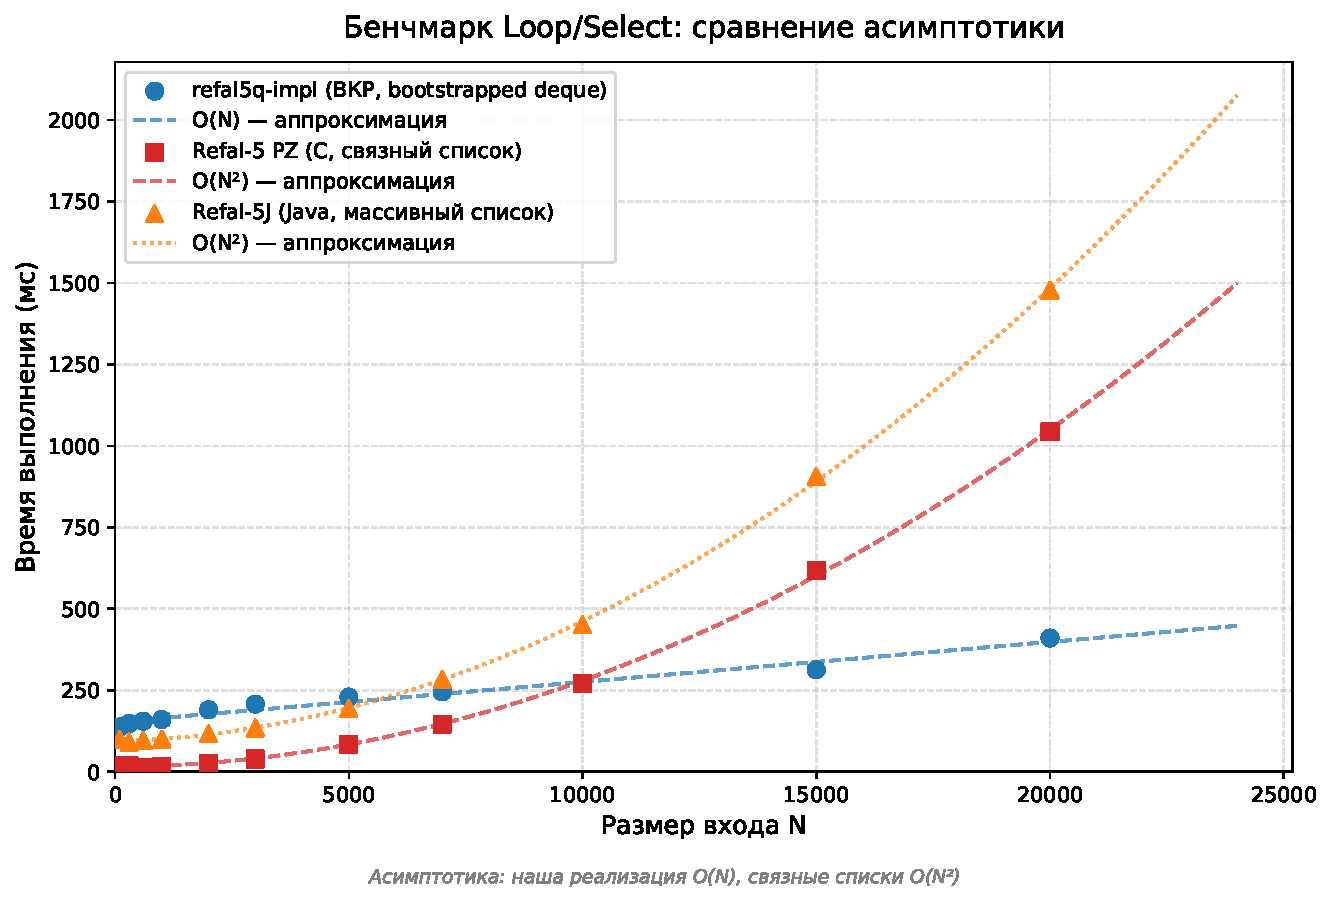
\includegraphics[width=0.95\textwidth]{loop-select-graph.pdf}
  \caption{Зависимость времени выполнения Loop/Select от размера входа N}
  \label{fig:bench-graph}
\end{figure}

\subsubsection{Тест на реальной программе: рассахариватель}

Loop/Select~--- синтетический тест: он нарочно нагружает ту единственную
операцию, на которой расходятся структуры данных. Чтобы проверить реализацию
на содержательной нагрузке, второй прогон выполнен на настоящей программе~---
рассахаривателе проекта \prog{refal-5-framework}~\cite{refal5_framework_github}.
Это пять модулей (\prog{desugar}, \prog{LibraryEx}, \prog{R5FW-Parser},
\prog{R5FW-Transformer}, \prog{R5FW-Plainer}) общим объёмом около 4200~строк;
на вход ему подаётся \prog{R5FW-Parser.ref}~--- сам синтаксический анализатор
рассахаривателя, 1038~строк, дающий на выходе около 45~КБ текста.

Один и тот же рассахариватель прогоняется тремя способами:
\begin{itemize}
  \item \prog{refal5q-impl}~--- наш интерпретатор исполняет пять
        рассахаренных \prog{.ref}-файлов напрямую;
  \item Refal-5~PZ~--- сначала компилирует \prog{.ref} в \prog{.rsl}
        (утилита \prog{refc}), затем исполняет (утилита \prog{refgo});
  \item Refal-5J~--- компилирует \prog{.ref} в \prog{.java}, затем в
        \prog{.class} (\prog{r5jc} + \prog{javac}) и запускает.
\end{itemize}

Все три реализации дают эквивалентный выход. Это и есть
главный результат теста: наш интерпретатор корректно исполняет реальную
программу такого объёма и воспроизводит поведение зрелых реализаций Рефала-5.

\subsubsection{Методика и результаты рассахаривателя}

Методика измерений совпадает с тестом Loop/Select: один прогревочный запуск
и три измеряемых, в отчёт идёт медиана. Для Refal-5~PZ и Refal-5J компиляция
выполняется один раз до замеров, поэтому измеряется только время исполнения
скомпилированной программы. Тайм-аут на один запуск~--- 300~секунд.

Запуск выполняется скриптом \prog{bench/desugar-bench.ps1}:

\begin{lstlisting}[language=bash,caption={Запуск бенчмарка рассахаривателя},label={lst:desugar-bench-run}]
powershell -File bench\desugar-bench.ps1 -WithPZ -WithR5J
\end{lstlisting}

Медианные времена приведены в таблице~\ref{tab:desugar-results}.

\begin{table}[!htb]
\caption{\centering Время рассахаривания R5FW-Parser.ref (мс, медиана 3 прогонов)}
\label{tab:desugar-results}
\centering
\small
\begin{tabular}{|l|r|l|}
\hline
\textbf{Реализация} & \textbf{Время, мс} & \textbf{Режим исполнения} \\
\hline
refal5q-impl & 2055 & интерпретация \\
\hline
Refal-5~PZ   & 369  & компиляция (refc + refgo) \\
\hline
Refal-5J     & 1632 & компиляция (r5jc + javac) \\
\hline
\end{tabular}
\end{table}

\subsubsection{Обсуждение результатов}

Два прогона отвечают на разные вопросы, поэтому обсудим их по очереди:
Loop/Select показывает, как ведёт себя структура данных под алгоритмической
нагрузкой, а рассахариватель~--- как реализация справляется с реальной
программой целиком.

Сначала о тесте Loop/Select.
На малых $N$ наша реализация проигрывает обоим конкурентам.
Причина простая: запуск JVM и прогрев JIT-компилятора стабильно стоят
около 120~мс, и эта плата не зависит от размера входа. Refal-5~PZ~---
нативный бинарник, его старт укладывается в единицы миллисекунд;
Refal-5J работает на той же JVM, что и мы, но тратит на инициализацию
порядка 85--90~мс.

При $N \approx 7000$ кривая Refal-5J уже догоняет нашу, при $N \approx 9000$
её перешагивает Refal-5~PZ. После этой точки квадратичный рост
конкурентов берёт своё: на $N = 10\,000$ PZ уже медленнее (277~мс против
254~мс), а на $N = 20\,000$ разрыв с PZ становится 3,5-кратным
(1059~мс против 302~мс) и 4,5-кратным с Refal-5J
(1348~мс против 302~мс).

Объяснение различия лежит в способе хранения объектного выражения.
Refal-5~PZ и Refal-5J держат выражение в виде двусвязного списка
термов: при построении нового скобочного терма \prog{(e.Acc A/B)}
на $k$-й итерации нужно скопировать всю накопленную часть длиной $k$.
$N$ итераций по $O(k)$ дают $O(N^2)$. Наш интерпретатор устроен иначе:
значение переменной идёт на стек одним объектом \prog{BulkPassive},
а сборка аргументов вызова использует \prog{Expr.concat}~--- по схеме
Окасаки это амортизированная константа независимо от длины операндов.
$N$ итераций по $O(1)$ дают $O(N)$~--- ровно то, что показывает прямая
на графике.

У замера есть границы применимости, и их стоит назвать прямо.
Меряется время жизни всего процесса, поэтому наши $\approx 120$~мс на $N = 100$~---
это почти целиком запуск JVM, а не работа интерпретатора. Диапазон $N$ до 20\,000
захватывает лишь начало параболы конкурентов: на больших $N$ разрыв рос бы быстрее, но
прогон при $N \sim 10^5$ уже упирается в тайм-аут 120~с. Наконец, PZ и Refal-5J в обоих
тестах выступают как компиляторы~--- компиляция сделана заранее, и замеряется только
исполнение готового кода, так что на Loop/Select мы сравниваем алгоритмические сложности
структур данных, а не режимы исполнения.

Теперь о тесте рассахаривателя.
И здесь конкуренты также работают как компиляторы: и Refal-5~PZ,
и Refal-5J сначала переводят программу в нативный код или байт-код, а потом
исполняют уже скомпилированное. Отличие от Loop/Select в том, что
рассахариватель не содержит квадратичного паттерна, поэтому алгоритмического
преимущества у нас нет, и они закономерно быстрее нашего интерпретатора~---
Refal-5~PZ в 5,6~раза, Refal-5J в 1,3~раза. Это не алгоритмический проигрыш,
а ожидаемая разница между компиляцией и интерпретацией: наша реализация на
каждом шаге заново разбирает поле зрения, тогда как скомпилированная программа
исполняет готовый код. Наибольший отрыв даёт Refal-5~PZ как нативный
компилятор; Refal-5J ближе к нам, потому что работает на той же JVM и платит
те же стартовые накладные расходы.

Важно, что главный вывод этого теста не про время, а про корректность: наш
интерпретатор исполняет программу в 4200~строк и выдаёт ровно тот же результат,
что зрелые реализации Рефала-5. Вместе два прогона дают согласованную картину.
На алгоритмически тяжёлом паттерне, где растущий аккумулятор многократно
копируется, выигрывает структура данных~--- раскрученная очередь даёт $O(N)$
там, где списочные представления дают $O(N^2)$. На обычной программе без
такого паттерна решает способ исполнения, и компиляция ожидаемо обходит
интерпретацию. Ни одно из наблюдений не противоречит другому: они измеряют
разные свойства реализации.

\anonsection{ЗАКЛЮЧЕНИЕ}
В рамках выпускной квалификационной работы поставлена и решена задача
разработки компилятора базисного подмножества Рефала-5 с представлением
объектных выражений на основе раскрученной двусторонней очереди, а также
подтверждения корректности и работоспособности реализации автоматическими
тестами и сравнительным прогоном с двумя альтернативными реализациями
языка.

В исследовательской части рассмотрены базовые понятия Рефала-5 и
существующие представления объектных выражений (классическое плоское
двусвязное, компромиссное с подвешенными скобками, массивное,
векторно-списковое и дерево конкатенаций), обсуждены их компромиссы по
ключевым операциям и обоснован выбор раскрученной двусторонней очереди по
Окасаки~\cite{okasaki_pfds} как структуры, амортизированно покрывающей все
основные операции (отделение терма с концов, конкатенацию и многократное
использование значения переменной).

В конструкторской части зафиксированы функциональные и нефункциональные
требования к системе, декомпозиция на модули с привязкой к Java-пакетам,
интерфейс контейнера выражения и требования к механизму сопоставления, выделены
точки расширения и определены классы ошибок с единым форматом
диагностических сообщений.

В технологической части реализован компилятор с интерпретирующим исполнением,
выполняющий лексический,
синтаксический и семантический анализ исходного текста и формирующий
внутреннее представление программы. Раскрученная двусторонняя очередь
реализована через запечатанный интерфейс \prog{Expr<T>} и пару классов
\prog{ShallowDeque<T>} (циклический массив фиксированной ёмкости
\(CAPACITY=9\)) и \prog{DeepDeque<T>} (тройка \(\langle front, mid, back
\rangle\) с рекурсивным средним уровнем); конкатенация со всеми четырьмя
случаями Shallow/Deep $\times$ Shallow/Deep вынесена в служебный класс
\prog{ExprOps}. Исполняющий модуль реализован как цикл нормализации в
прикладном порядке с сопоставлением образца через перебор длины
\(e\)-переменной и сборкой результата через \prog{Expr.concat}. Реализован
минимальный набор встроенных функций (ввод-вывод, арифметика, работа со
строками и символами, функции высшего порядка), достаточный для тестовых
программ и для выхода рассахаривателя \prog{r5fw-desugar} проекта
\prog{refal-5-framework}~\cite{refal5_framework_github}; директива
\prog{\$EXTERN} поддерживается, что обеспечивает совместимость с этим
рассахаривателем.

В аналитической части построен автоматический набор из \(224\) тестов:
\(143\) теста JUnit~5~\cite{junit5_guide}, покрывающих лексер, парсер,
семантический анализ, сопоставление, подстановку, цикл нормализации и саму
раскрученную очередь, и \(81\) внешняя программа в рамках
\prog{AutotestsRunnerTest}~--- фикстуры из репозиториев
\prog{refal-5j} и \prog{refal-5-framework}~\cite{refal5_framework_github}.
Среднее покрытие по инструкциям байт-кода составляет около \(87\,\%\),
по веткам~--- около \(77\,\%\), что выше зафиксированных в \prog{pom.xml} порогов.
Дополнительно проведены два сравнительных прогона трёх реализаций Рефала-5
(\prog{refal5q-impl}, Refal-5~PZ~\cite{refal5_home} и Refal-5J): синтетический
тест Loop/Select и прогон рассахаривателя \prog{R5FW-Parser.ref} из проекта
\prog{refal-5-framework}~\cite{refal5_framework_github}. Замеры автоматизированы
скриптами \prog{bench/loop-select-bench.ps1} и \prog{bench/desugar-bench.ps1};
методика~--- один прогревочный запуск и три измеряемых, в отчёт идёт медиана.

Основные численные результаты: автоматический прогон \prog{mvn clean
verify} проходит без нарушений; контроль стиля Checkstyle и
покрытие выполняются выше установленных порогов. На тесте Loop/Select
на малых $N$ разработанная реализация проигрывает конкурентам из‑за
накладных расходов запуска JVM ($\approx 120$~мс), однако при росте входа
зависимость времени от $N$ остаётся линейной: при $N = 20\,000$ время
составляет 302~мс против 1059~мс у Refal-5~PZ и 1348~мс у Refal-5J
(разрыв 3,5 и 4,5~раза соответственно). На прогоне рассахаривателя все
три реализации выдают эквивалентный результат; по времени Refal-5~PZ
быстрее в 5,6~раза, Refal-5J~--- в 1,3~раза, что соответствует ожидаемому
преимуществу компиляции над интерпретацией на программе без квадратичного
паттерна.

Возможные направления дальнейшего развития системы:

\begin{itemize}
  \item Компиляция в JVM-байт-код по образцу Refal-5J: порождение для
        каждого правила отдельного Java-метода уменьшило бы постоянный
        множитель и сократило бы отставание от Refal-5J на программах
        без квадратичного паттерна, например на прогоне рассахаривателя.
  \item Поддержка модульной системы Рефала-5 (директива \prog{*\$FROM},
        квалифицированные имена). Текущая реализация поддерживает
        конкатенацию нескольких файлов через синтаксис \prog{+}, однако
        \prog{*\$FROM} и квалифицированные имена функций не реализованы.
  \item Расширение библиотеки встроенных функций до полного набора
        Рефал-5 (\prog{Br}/\prog{Dg}, шифр-функции, файловый ввод-вывод).
        Архитектура регистрации позволяет это сделать без изменений ядра.
\end{itemize}

\indent Полученная программная система (Maven-проект \prog{refal5q-impl} объёмом
\(\sim 3\,800\) строк основного кода и \(\sim 1\,700\) строк тестов) может
использоваться как самостоятельный компилятор базисного подмножества
Рефала-5 и как базовая платформа для дальнейших исследований в области
эффективных представлений объектных выражений и компиляции функциональных
языков переписывания термов.


\newpage
\phantomsection
\addcontentsline{toc}{section}{СПИСОК ИСПОЛЬЗОВАННЫХ ИСТОЧНИКОВ}%
\centeredsection{СПИСОК ИСПОЛЬЗОВАННЫХ ИСТОЧНИКОВ}
\printbibliography[heading=none]

\appendix
\setcounter{subsection}{0}
\renewcommand{\thesubsection}{}
\clearpage

\anonsection{ПРИЛОЖЕНИЕ А}
\label{app:grammar}

\subsection*{Формальная грамматика базисного подмножества Рефала-5}

Грамматика приведена в нотации EBNF. Синтаксис базисного подмножества является
точным подмножеством синтаксиса Рефала-5. В реализуемом базисном подмножестве дополнительно
поддерживается директива \prog{\$EXTERN}, нужная для согласованности с выходом
рассахаривателя \prog{r5fw-desugar}~\cite{refal5_framework_github}.

\subsection*{Лексика}

\begin{itemize}
  \item Пробелы и переводы строк разделяют токены и игнорируются.
  \item Комментарий: строка, начинающаяся с \prog{*}, до конца строки.
  \item Целое число: \prog{-?[0-9]+}.
  \item Строка: \prog{'\ldots'} либо \prog{\textquotedbl\ldots\textquotedbl} (без экранирования; допускаются любые
        символы до следующей кавычки того же вида).
  \item Идентификатор: \prog{[A-Za-z.\_\$][A-Za-z0-9.\_\$\-]*}.
  \item Зарезервированные директивы: \prog{\$ENTRY}, \prog{\$EXTERN}.
  \item Скобки и разделители: \prog{\{ \} ( ) < > = ; ,}.
\end{itemize}

\subsection*{Синтаксис (EBNF)}

\begin{lstlisting}[language={},caption={EBNF-грамматика базисного подмножества Refal-5},label={lst:ebnf}]
Program     ::= TopLevel* EOF ;

TopLevel    ::= EntryDecl | ExternDecl | FuncDef ;

EntryDecl   ::= "$ENTRY" Ident ";"
              | "$ENTRY" FuncDef ;

ExternDecl  ::= "$EXTERN" Ident ("," Ident)* ";" ;

FuncDef     ::= Ident "{" Rule+ "}" ;

Rule        ::= Pattern "=" Result ";"? ;

Pattern     ::= PatternTerm* ;
PatternTerm ::= Int | Str | QuotedSym | Var | "(" PatternTerm* ")" ;

Result      ::= ResultTerm* ;
ResultTerm  ::= Int | Str | QuotedSym | Var | Symbol
              | "(" ResultTerm* ")"
              | "<" Ident ResultTerm* ">" ;

Var         ::= ("s" | "t" | "e") "." VarName ;
VarName     ::= (Letter | Digit | "_" | "." | "$")+ ;

Symbol      ::= Ident ;
Ident       ::= Letter (Letter | Digit | "_" | "-" | "+" | ".")* ;
Int         ::= Digit+ ;
Str         ::= '"' Char* '"' ;
QuotedSym   ::= "'" Char* "'" ;
\end{lstlisting}

\subsection*{Семантика сопоставления}

\begin{itemize}
  \item \prog{s.X}~--- связывается с ровно одним \emph{атомарным} термом (символ, число или
        строка); скобочный терм не подходит.
  \item \prog{t.X}~--- связывается с ровно одним термом (включая скобочный).
  \item \prog{e.X}~--- связывается с последовательностью термов (возможно пустой).
  \item Если переменная встречается в правиле несколько раз~--- все вхождения должны быть
        связаны с одинаковыми значениями.
  \item В теле функции выбирается \emph{первое} правило, чей образец сопоставим с
        аргументами; затем результат подставляется и редуцируется.
\end{itemize}

\subsection*{Что \emph{не} поддерживается}

\begin{itemize}
  \item Условия \prog{,~e.Cond} после паттерна, блоки \prog{\{ : \}}~--- для них применяется
        внешний рассахариватель \prog{r5fw-desugar}, выход которого уже укладывается в эту
        грамматику.
  \item Экранирование в строках (\prog{\textbackslash n}, \prog{\textbackslash x42}).
  \item Макроцифры \prog{@BIG-MACRODIGIT@}.
  \item Псевдокомментарии \prog{*\$CLASSIC} / \prog{*\$EXTENDED}.
  \item Декларации \prog{*\$FROM} (директива модульной системы Рефала-5); несколько файлов
        загружаются через синтаксис \prog{+}: \prog{java -jar target/refal5q.jar a.ref+b.ref+c.ref}.
\end{itemize}

\clearpage
\anonsection{ПРИЛОЖЕНИЕ Б}
\label{app:listings}

\subsection*{Листинги ключевых функций}

В приложении приведены ключевые фрагменты исходного кода Java-реализации
с пояснительными комментариями. Каждый листинг сопровождён ссылкой на
соответствующий файл в каталоге \prog{refal5q-impl/src/main/java/refal/}.

\subsection*{Конкатенация контейнеров ExprOps.concat}

Файл \prog{refal5q-impl/src/main/java/refal/deque/ExprOps.java}.

\begin{lstlisting}[language=Java,caption={Конкатенация двух Expr с разбором всех четырёх случаев},label={lst:app-concat}]
static <T> Expr<T> concat(Expr<T> a, Expr<T> b) {
    if (a.isEmpty()) return b;
    if (b.isEmpty()) return a;
    if (a instanceof ShallowDeque<T> sa && b instanceof ShallowDeque<T> sb) return concatSS(sa, sb);
    if (a instanceof ShallowDeque<T> sa && b instanceof DeepDeque<T> db)    return concatSD(sa, db);
    if (a instanceof DeepDeque<T> da && b instanceof ShallowDeque<T> sb)    return concatDS(da, sb);
    DeepDeque<T> da = (DeepDeque<T>) a;
    DeepDeque<T> db = (DeepDeque<T>) b;
    return concatDD(da, db);
}

private static <T> Expr<T> concatDD(DeepDeque<T> a, DeepDeque<T> b) {
    int total = a.size() + b.size();
    ShallowDeque<T> ab = a.back();
    ShallowDeque<T> bf = b.front();
    int boundary = ab.size() + bf.size();

    Expr<ShallowDeque<T>> aMidPlus = a.mid();
    if (boundary == 0) {
        (*@{\color{black}\ttfamily // оба граничных буфера пусты -- ничего добавлять не нужно.}@*)
    } else if (boundary <= CAPACITY) {
        ShallowDeque<T> merged = ShallowDeque.empty();
        for (T x : iter(ab)) merged = merged.pushBackTight(x);
        for (T x : iter(bf)) merged = merged.pushBackTight(x);
        aMidPlus = aMidPlus.pushBack(merged);
    } else {
        Object[] tmp = new Object[boundary];
        int i = 0;
        for (T x : iter(ab)) tmp[i++] = x;
        for (T x : iter(bf)) tmp[i++] = x;
        int rightLen = boundary - CAPACITY;
        if (rightLen < ShallowDeque.MIN_FILL) rightLen = ShallowDeque.MIN_FILL;
        int leftLen = boundary - rightLen;
        ShallowDeque<T> m1 = ShallowDeque.ofArray(tmp, 0, leftLen);
        ShallowDeque<T> m2 = ShallowDeque.ofArray(tmp, leftLen, rightLen);
        aMidPlus = aMidPlus.pushBack(m1).pushBack(m2);
    }

    Expr<ShallowDeque<T>> newMid = concat(aMidPlus, b.mid());
    return DeepDeque.mkDeep(a.front(), newMid, b.back(), total);
}
\end{lstlisting}

Случай Deep+Deep явно показан полностью --- в нём проявляется рекурсивный
вызов \prog{concat} на средних очередях буферов, обеспечивающий
амортизированно \(O(1)\) сложность по Окасаки~\cite{okasaki_pfds}. Случаи
Shallow+Shallow, Shallow+Deep и Deep+Shallow (методы \prog{concatSS},
\prog{concatSD}, \prog{concatDS}) реализованы аналогично с расщеплением
объединённого буфера ровно пополам, если он превышает \prog{CAPACITY}.

\subsection*{Сопоставление образца с выражением Matcher.match}

Файл \prog{refal5q-impl/src/main/java/refal/runtime/Matcher.java}.

\begin{lstlisting}[language=Java,caption={Сопоставление образца с выражением (с backtracking по e-переменным)},label={lst:app-match}]
public static Optional<Bindings> match(List<Term> pattern, List<Term> expr) {
    return rec(pattern, 0, expr, 0, expr.size(), Bindings.empty());
}

private static Optional<Bindings> rec(
        List<Term> pat, int pi,
        List<Term> exp, int ei, int eEnd,
        Bindings env) {
    if (pi == pat.size()) {
        return ei == eEnd ? Optional.of(env) : Optional.empty();
    }
    Term p = pat.get(pi);

    if (p instanceof Var v && v.kind() == 'e') {
        String key = v.key();
        if (env.contains(key)) {
            (*@{\color{black}\ttfamily // Повторное вхождение: проверяем совпадение.}@*)
            List<Term> bound = env.get(key);
            int len = bound.size();
            if (ei + len > eEnd) return Optional.empty();
            for (int k = 0; k < len; k++) {
                if (!exp.get(ei + k).equals(bound.get(k))) return Optional.empty();
            }
            return rec(pat, pi + 1, exp, ei + len, eEnd, env);
        }
        (*@{\color{black}\ttfamily // Свежая e.X -- перебираем длину захвата 0, 1, ...}@*)
        for (int len = 0; ei + len <= eEnd; len++) {
            List<Term> chunk = exp.subList(ei, ei + len);
            Bindings env1 = env.with(key, List.copyOf(chunk));
            Optional<Bindings> r = rec(pat, pi + 1, exp, ei + len, eEnd, env1);
            if (r.isPresent()) return r;
        }
        return Optional.empty();
    }

    if (ei >= eEnd) return Optional.empty();
    Term x = exp.get(ei);

    if (p instanceof Var v) {
        String key = v.key();
        if (v.kind() == 's') {
            if (x instanceof Br) return Optional.empty();
            if (env.contains(key)) {
                List<Term> bound = env.get(key);
                if (bound.size() != 1 || !bound.get(0).equals(x)) return Optional.empty();
                return rec(pat, pi + 1, exp, ei + 1, eEnd, env);
            }
            return rec(pat, pi + 1, exp, ei + 1, eEnd, env.with(key, List.of(x)));
        }
        if (v.kind() == 't') {
            if (env.contains(key)) {
                List<Term> bound = env.get(key);
                if (bound.size() != 1 || !bound.get(0).equals(x)) return Optional.empty();
                return rec(pat, pi + 1, exp, ei + 1, eEnd, env);
            }
            return rec(pat, pi + 1, exp, ei + 1, eEnd, env.with(key, List.of(x)));
        }
    }

    if (p instanceof Br pBr) {
        if (!(x instanceof Br xBr)) return Optional.empty();
        Optional<Bindings> inner = rec(pBr.items(), 0, xBr.items(), 0, xBr.items().size(), env);
        if (inner.isEmpty()) return Optional.empty();
        return rec(pat, pi + 1, exp, ei + 1, eEnd, inner.get());
    }

    if (p.equals(x)) return rec(pat, pi + 1, exp, ei + 1, eEnd, env);
    return Optional.empty();
}
\end{lstlisting}

\subsection*{Подстановка результата правила Substitutor.substitute}

Файл \prog{refal5q-impl/src/main/java/refal/runtime/Substitutor.java}.

\begin{lstlisting}[language=Java,caption={Сборка результата правила через Expr.concat},label={lst:app-subst}]
public static Expr<Term> substitute(List<Term> result, Bindings env) {
    Expr<Term> out = Expr.empty();
    for (Term t : result) {
        switch (t) {
            case Var v -> {
                String key = v.key();
                if (!env.contains(key)) {
                    throw new IllegalStateException(
                            "Unbound variable in result: " + key);
                }
                out = Expr.concat(out, Expr.fromList(env.get(key)));
            }
            case Br br -> {
                Expr<Term> inner = substitute(br.items(), env);
                out = out.pushBack(new Br(inner.toList()));
            }
            case Call c -> {
                Expr<Term> argDq = substitute(c.args(), env);
                out = out.pushBack(new Call(c.fn(), argDq.toList()));
            }
            default -> out = out.pushBack(t);
        }
    }
    return out;
}
\end{lstlisting}

Использование switch-выражения с шаблонами над запечатанным
интерфейсом \prog{Term} обеспечивает компилируемую полноту разбора:
если в иерархию AST добавляется новый вид терма, компилятор Java потребует
обработать его явно.

\subsection*{Цикл нормализации Runtime.normalize и Runtime.evalCall}

Файл \prog{refal5q-impl/src/main/java/refal/runtime/Runtime.java}.

\begin{lstlisting}[language=Java,caption={Цикл нормализации (прикладной порядок, сначала крайний слева)},label={lst:app-normalize}]
public Expr<Term> normalize(Expr<Term> expr) {
    Expr<Term> out = Expr.empty();
    for (Term t : expr) {
        out = Expr.concat(out, normalizeTerm(t));
    }
    return out;
}

private Expr<Term> normalizeTerm(Term t) {
    return switch (t) {
        case Call c -> {
            bumpStep();
            Expr<Term> normalizedArgs = normalize(Expr.fromList(c.args()));
            Expr<Term> body = evalCall(c.fn(), normalizedArgs.toList());
            yield normalize(body);
        }
        case Br br -> {
            Expr<Term> inner = normalize(Expr.fromList(br.items()));
            yield Expr.singleton(new Br(inner.toList()));
        }
        default -> Expr.singleton(t);
    };
}

public Expr<Term> evalCall(String fn, List<Term> args) {
    BuiltinFn b = builtins.get(fn);
    if (b != null) {
        List<Term> r = b.apply(this, args);
        return Expr.fromList(r);
    }
    Optional<Func> f = program.getFunc(fn);
    if (f.isEmpty()) {
        throw new RefalException("Unknown function: " + fn);
    }
    for (Rule rule : f.get().rules()) {
        var bindings = Matcher.match(rule.pattern(), args);
        if (bindings.isPresent()) {
            return Substitutor.substitute(rule.result(), bindings.get());
        }
    }
    throw new RefalException("No matching rule for " + fn + " on args=" + args);
}
\end{lstlisting}

\clearpage
\anonsection{ПРИЛОЖЕНИЕ В}
\label{app:reproduce}

\subsection*{Команды воспроизведения тестов и сравнительного прогона}

Все команды выполняются из каталога \prog{refal5q-impl/}. Предполагаются
установленными Java~25~LTS~\cite{java_se25_spec} (с
переменной \prog{JAVA\_HOME}, указывающей на JDK) и Apache Maven~3.9 или
выше~\cite{maven_guide}.

\subsection*{Установка инструментов}

\begin{lstlisting}[language=bash,caption={Проверка инструментов перед сборкой}]
$ java -version       (*@{\color{black}\ttfamily \# ожидается 25.x}@*)
$ javac -version      (*@{\color{black}\ttfamily \# ожидается 25.x}@*)
$ mvn -version        (*@{\color{black}\ttfamily \# ожидается 3.9.x или новее}@*)
\end{lstlisting}

Зависимости проекта (JUnit~5, AssertJ, JaCoCo, Checkstyle) подтягиваются
Maven автоматически из локального репозитория \prog{\textasciitilde/.m2/}; явная
установка не требуется.

\subsection*{Полная сборка с тестами и проверками}

\begin{lstlisting}[language=bash,caption={Полная сборка проекта}]
$ mvn clean verify
\end{lstlisting}

Команда выполняет:
\begin{itemize}
  \item компиляцию (\prog{maven-compiler-plugin}, целевой релиз --- 25);
  \item запуск всех \(143\) тестов JUnit~5 (\prog{maven-surefire-plugin});
  \item построение самодостаточного JAR-файла \prog{target/refal5q.jar} (\prog{maven-shade-plugin});
  \item проверку покрытия (\prog{jacoco-maven-plugin}; пороги
        \(\geq 70\,\%\) по инструкциям и \(\geq 55\,\%\) по веткам для
        пакетов \prog{refal.deque} и \prog{refal.runtime});
  \item проверку стиля кода (\prog{maven-checkstyle-plugin}, конфигурация
        \prog{checkstyle.xml}).
\end{itemize}

При успешном завершении в каталоге \prog{target/site/jacoco/} лежит HTML-отчёт о
покрытии, в \prog{target/} --- jar-артефакт.

\subsection*{Запуск программы}

\begin{lstlisting}[language=bash,caption={Запуск программы из файла}]
$ java -jar target/refal5q.jar bench/hello.ref --expr "'World'"
\end{lstlisting}

При наличии \prog{\$ENTRY} в файле опция \prog{--entry} необязательна.
Опция \prog{--step-limit~N} устанавливает лимит шагов редукции
(по умолчанию \(100\,000\)).

\subsection*{Workflow с внешним рассахаривателем}

Если исходный файл написан с использованием расширенного синтаксиса
Рефала-5 (условия \prog{,~e.Cond}, блоки \prog{\{ : \}}), то перед запуском
его пропускают через рассахариватель из проекта
\prog{refal-5-framework}~\cite{refal5_framework_github}:

\begin{lstlisting}[language=bash,caption={Полный workflow с рассахаривателем}]
$ refgo r5fw-desugar program.ref program-desugared.ref
$ java -jar target/refal5q.jar program-desugared.ref --entry Go
\end{lstlisting}

\subsection*{Сравнительные прогоны трёх реализаций Рефала-5}

Сравнительные прогоны из подраздела~\ref{subsec:benchmarks} автоматизированы
двумя PowerShell-скриптами. Оба ожидают установленный Refal-5~PZ~\cite{refal5_home}
(дистрибутив Version~PZ с сайта ИПМ им.~А.~П.~Ершова; пути к
\prog{refgo.exe} и \prog{refc.exe} задаются в начале скрипта) и опционально~---
Refal-5J при включённой опции \prog{-WithR5J}.

Скрипт \prog{bench/loop-select-bench.ps1} прогоняет синтетический тест
Loop/Select при значениях $N$ от 100 до 20\,000:

\begin{lstlisting}[language=bash,caption={Запуск бенчмарка Loop/Select}]
$ powershell -File bench\loop-select-bench.ps1 -WithPZ -WithR5J
\end{lstlisting}

Скрипт \prog{bench/desugar-bench.ps1} измеряет время рассахаривания
\prog{R5FW-Parser.ref}:

\begin{lstlisting}[language=bash,caption={Запуск бенчмарка рассахаривателя}]
$ powershell -File bench\desugar-bench.ps1 -WithPZ -WithR5J
\end{lstlisting}

По умолчанию выполняется \(1\) прогревочный запуск и \(3\) измеряемых, в
отчёт идёт медиана; параметры регулируются опциями \prog{-WarmupRuns} и
\prog{-MeasuredRuns}. Результаты Loop/Select сохраняются в
\prog{bench/loop-select-results.csv}; график для основного текста строится
отдельно командой \prog{python bench/plot-benchmark.py --out bench/loop-select-graph.pdf}.
Время рассахаривания записывается в \prog{bench/desugar-results.csv}.

\clearpage
\anonsection{ПРИЛОЖЕНИЕ Г}
\label{app:loopselect-src}

\subsection*{Исходный код теста Loop/Select}

Тестовая программа сравнительного прогона из подраздела~\ref{subsec:benchmarks}.
Файл \prog{refal5q-impl/bench/loop-select.ref}. Аргумент \prog{<Arg 1>}~---
число итераций $N$; на каждой итерации функция \prog{Loop} строит новый
скобочный терм из растущего аккумулятора \prog{e.Acc}, а \prog{Select}
выбирает одну из двух альтернатив в зависимости от направления.

\begin{lstlisting}[language=Refal,caption={Тестовая программа Loop/Select},label={lst:app-loopselect}]
$ENTRY Go {
  = <TimeElapsed 0>
    <Loop Left () <Numb <Arg 1>>>
    <Prout <TimeElapsed>>;
}

Loop {
  s.Side (e.Acc) 0 = /* done */;
  s.Side (e.Acc) s.Rest
    = <Loop <Select s.Side (e.Acc A) (e.Acc B)> <- s.Rest 1>>;
}

Select {
  Left  t.Left t.Right = Right t.Left;
  Right t.Left t.Right = Left  t.Right;
}
\end{lstlisting}


\end{document}
